\documentclass[a4paper]{abnt}
\usepackage[utf8]{inputenc}
\usepackage[T1]{fontenc}
\usepackage[brazilian]{babel}
\usepackage{graphicx}
\usepackage{xcolor}
\usepackage{epigraph}
\usepackage{booktabs}
\usepackage{listings}
\usepackage[footnote]{acronym}
\usepackage[hyperindex=false]{hyperref}
\usepackage{tabela-simbolos}
\usepackage[alf]{abntcite}
\usepackage{amssymb}
\usepackage[boxed,portugues]{algorithm2e}
\usepackage{verbatim}
\usepackage{multirow}
\usepackage{tabularx}
\usepackage{longtable}
\usepackage{colortbl}
\usepackage{subfig}

\pdfimageresolution=300

\hyphenation{heu-rís-ti-cas}
\hyphenation{pré-con-fi-gu-ra-ção}
\hyphenation{DVFSMachine}

\renewcommand{\familydefault}{\sfdefault}
\def \r{\textsuperscript{\textregistered}}

\renewcommand\lstlistingname{Texto C++}
\lstset{language=C++, frame=single, extendedchars=false}

\newcolumntype{C}{>{\centering\arraybackslash}X}

\usepackage{ifpdf}

\titulo{Real-Time Dynamic Voltage and Frequency Scaling no sistema EPOS}
\autor{Gustavo Roberto Nardon Meira}
\orientador{Prof. Dr. Antônio Augusto Medeiros Fröhlich}
\coorientador{Arliones Hoeller Júnior, Me.}
\instituicao{Universidade Federal de Santa Catarina \par
    Centro Tecnológico \par
    Departamento de Informática e Estatística}
\comentario{Apresentado como requisito à obtenção do grau de Bacharel em Ciência da Computação}
\data{31 de outubro de 2011}

\lstset{
    tabsize=2,
    basicstyle=\footnotesize,
}

%%%%
%%%%
%%%% ALTERAR A DATA ABAIXO: 
%%%%
%%%%

\begin{document}
    \capa
    \folhaderosto

    \setlength{\ABNTsignthickness}{0.4pt}
    \begin{folhadeaprovacao}
        Monografia sob o título
        ``Real-Time Dynamic Voltage and Frequency Scaling no sistema EPOS'', defendida
        em 4 de outubro de 2011 por Gustavo Roberto Nardon Meira, como parte dos requisitos à obtenção
        do grau de Bacharel em Ciência da Computação, e aprovada pela seguinte banca examinadora:
    
        \assinatura{Prof. Dr. Antônio Augusto M. Fröhlich \\ Orientador}
        \assinatura{Prof. Dr. Rafael Luiz Cancian}
        \assinatura{Me. Giovani Gracioli}
    \end{folhadeaprovacao}
       
    
    %\begin{titlepage}
    %    \vspace*{20cm}
    %    \epigraph{Em breve seu concorrente anunciará aqui\ldots}{Lista telefônica EMBRATEL}
    %\end{titlepage}


    %\begin{abstract}
    % First we need a resumo... 
    %\end{abstract}
    
    % 1. Autonomia de sistemas EMBARCADOS móveis é um problema.
    % 2. DVS é uma técnica assim assado.
    % 3. DVS tem se mostrado boa em resolver este problema em sistemas embarcados.
    % 4. Se colocarmos RT, fode tudo!
    % 5. O que este trabalho faz é...
        
    \begin{resumo}
    
        \emph{Dynamic Voltage and Frequency Scaling} (DVFS) é uma técnica de gerenciamento de energia que permite ao sistema operacional decidir quando alterar a tensão e frequência do processador, sendo possível reduzir o desempenho e consumo de energia durante uma baixa demanda computacional. Em sistemas embarcados, além do tempo de vida de bateria, muitas vezes responder em tempo real também se torna uma restrição. Nesse cenário, economizar energia em detrimento do desempenho nem sempre pode ser uma boa ideia. Explorando este problema, o presente trabalho porta o sistema operacional embarcado de tempo real EPOS para a plataforma Intel PXA255, que permite o uso de DVFS. Além disso, um suporte a heurísticas para adequação de desempenho também foi criado. Os experimentos realizados demonstram a economia de energia sem que as tarefas do sistema percam prazos.

        % \emph{Dynamic Voltage and Frequency Scaling} (DVFS) é uma técnica que, explorando as propriedades elétricas dos processadores atuais, pode reduzir o consumo de energia do circuito através da diminuição de sua tensão e frequência de funcionamento. Assim, um sistema operacional ciente desta característica pode estabelecer um contrato entre a energia utilizada e desempenho. Tratando-se de aplicações embarcadas, além do tempo de vida da possível bateria, muitas vezes a obtenção de repostas em tempo real torna-se também uma restrição. Neste cenário, economizar energia em detrimento do desempenho nem sempre pode ser uma boa ideia, impedindo, por exemplo, que uma tarefa de tempo real seja executada dentro de seu prazo. Explorando este problema, o presente trabalho propõe o porte do EPOS para uma plataforma de hardware com suporte a DVFS, e ainda a implementação de heurísticas capazes de reduzir o consumo de energia utilizando a alteração de tensão e frequência do processador, de modo que tarefas de tempo real ainda possam responder em tempo hábil.
        
    % O Cancian comentou que "vale a pena citar aqui as principais características desses escalonadores", o que não sei se é uma boa ideia, pois acho que deixaria o resumo muito específico. Eu teria que falar de heurísticas estáticas e dinâmicas, explicar que elas exploram o slack ou a utilização de CPU.
        
    \end{resumo}

    \sumario
    \listoffigures
    \listoftables
    \listofalgorithms
    %\listadesiglas

    \acresetall

    \section{Introdu��o}


%- Ger�ncia de energia � importante para sistemas embarcados

Sistemas embarcados s�o plataformas computacionais dedicados a executar um
determinado conjunto de tarefas com objetivos espec�ficos, como
monitorar e/ou controlar os ambientes nos quais est�o inseridos. Normalmente, 
esses sistemas apresentam rigorosas limita��es em termos das capacidades de 
processamento e de mem�ria. Al�m disso, muitos deles, devido � 
natureza m�vel das suas aplica��es, s�o alimentados por baterias com uma
limitada carga de energia. Essas limita��es fazem com que uma ger�ncia eficiente
do consumo de energia e que n�o ocasione interfer�ncia significativa 
na execu��o da aplica��o seja utilizada.

%- Ger�ncia em outros trabalhos (economizam energia). Nao eh suficiente...

O \emph{hardware} dos sistemas embarcados disponibiliza diferentes 
mecanismos para realizar a ger�ncia do consumo de energia. Dentre eles, 
os mais conhecidos s�o as t�cnicas de \textsc{DVS} (Dynamic Voltage
Scaling)~\cite{Pouwelse:2001,Weiser:1994} e 
hiberna��o de recursos~\cite{Kravets:1998,Helmbold:1996,Flinn:1999}.
%e conjuntos de distintos modos de opera��o (CITAR).
Alguns trabalhos na literatura exploram a integra��o dessas t�cnicas com
abordagens que garantem \QoS{} (\qos{}). A maioria dessas abordagens,
entretanto, apenas busca minimizar o consumo de energia com o foco 
principal nas m�tricas tradicionais de \qos{}, como para processamento, 
mem�ria e comunica��o. 
Como apresentado em um trabalho anterior~\cite{Wiedenhoft:WTR:2007}, n�s
argumentamos que n�o � suficiente apenas garantir m�tricas tradicionais de
\qos{} se a carga da bateria termina antes do t�rmino das tarefas.

%- Neste trabalho a id�ia � utilizar a energia como par�metro de QoS (citar meus artigos) para atender o tempo de dura��o do sistema e al�m disso atender os \deadlines{} temporais das tarefas de tempo real.

Neste trabalho utilizamos a energia como um novo par�metro de \qos{} para
atender o tempo de dura��o do sistema especificado pelo usu�rio, ou seja, 
\qos{} em termos de energia. Nos propomos,
tamb�m, a garantir os \deadlines{} das tarefas \emph{hard} pela sua 
import�ncia em sistemas embarcados de tempo real. 
A proposta desta abordagem � garantir a energia e os \deadlines{} das
tarefas \emph{hard} de tempo real, n�o com o objetivo de minimizar o consumo de
energia, mas otimizar a funcionalidade do sistema.

%- Como fazer? - usando t�cnicas da computa��o imprecisa (explicar o que �)

Para alcan�ar nosso objetivo, o controle de \qos{} foi inspirado na computa��o
imprecisa~\cite{Liu:1994,Lin:1987a,Lin:1987b}. A computa��o imprecisa divide as
tarefas em duas partes: uma com o fluxo obrigat�rio e outra com o fluxo
opcional. O fluxo obrigat�rio � a parte \emph{hard} da tarefa, e deve sempre 
ser executado com o seu \deadline{} atendido. O fluxo opcional � a parte
``melhor esfor�o'' da tarefa, e caso seja necess�rio, � poss�vel que n�o seja 
executado. A partir desse conceito de divis�o, o escalonador da computa��o
imprecisa impede a execu��o das partes opcionais quando existe a possibilidade
do \deadline{} de 
alguma parte obrigat�ria n�o ser atendido, e assim, reduz a demanda por
processamento do sistema. No nosso escalonador, al�m dessa possibilidade, 
propomos que as partes opcionais n�o sejam escalonadas quando o n�vel de energia
n�o ser� suficiente para atender o tempo especificado pela aplica��o.
Esse controle cria per�odos ociosos no sistema, que permite ao escalonador
usar t�cnicas de ger�ncia de energia para diminuir o consumo dos componentes
durante os per�odos ociosos criados.

%- Prot�tipo no EPOS e escalonador EDF...

O escalonador proposto � baseado no escalonador \textsc{EDF} 
(\emph{Earliest Deadline
First})~\cite{Liu:1973} para garantir os \deadlines{} das tarefas, no qual 
as tarefas com maiores \deadlines{} possuem menores prioridades.
Um prot�tipo desta proposta foi implementado no
\epos{}~\cite{Marcondes:ETFA:2006}, um sistema operacional embarcado baseado em
componentes. \epos{} disponibiliza um conjunto de mecanismos para a ger�ncia do
consumo de energia, desde uma infra-estrutura que permite as aplica��es 
realizarem a apropriada ger�ncia~\cite{Hoeller:DIPES:2006}, at� um 
gerente com diferentes modos de opera��o que realiza a ger�ncia para a
aplica��o~\cite{Wiedenhoft:ETFA:2007}. 
Al�m desses mecanismos, o \epos{} possui um
sistema de monitoramento da carga da bateria, que informa a energia
restante.%(CITAR RAPHAEL).

%- Divis�o das se��es

Este artigo � estruturado como segue. Se��o~\ref{sc:relacionados} apresenta os
trabalhos relacionados. Se��o~\ref{sc:proposta} descreve o escalonador
desenvolvido neste trabalho, com a sua devida formaliza��o. 
Se��o~\ref{sc:implementacao} abrange a implementa��o do ambiente da computa��o
imprecisa e do escalonador proposto no sistema operacional embarcado escolhido.
Se��o~\ref{sc:conclusao} finaliza com a conclus�o do artigo.
%e apresenta as  futuras dire��es para este trabalho.


    \chapter{Fundamentação}
    \label{chap:fundamentacao}
    
    Este capítulo apresenta os fundamentos necessários para o entendimento do desenvolvimento do trabalho. As duas primeiras seções abordam os conceitos de tempo real e DVFS utilizados. A terceira e última seção aborda estes dois primeiros conceitos somados, apresentando então a ideia de DVFS em tempo real.
    
    \section{Sistema de Tempo Real}
        \label{sec:sistema-de-tempo-real}
        
        Esta seção apresenta o modelo de sistema de tempo real que será utilizado neste trabalho. Ele é baseado diretamente no modelo que \citeonline{Pillai:2001} utilizam para propor as heurísticas escolhidas para implementação. Neste cenário, um sistema de tempo real é um conjunto de tarefas periódicas com prazos definidos, todas concorrendo por um único processador. Ainda, para os efeitos deste trabalho, as tarefas apresentadas são passíveis de preempção, ou seja, a qualquer momento podem ser interrompidas para que cedam o uso processador.
    
        \subsection{Modelo de Sistema de Tempo Real}
            \label{sec:modelo-de-sistema-de-tempo-real}
    
        No modelo em questão, o sistema é composto por um conjunto de tarefas periódicas que não compartilham nenhum recurso entre si. Assim sendo, a toda tarefa $T_i$, tem-se atribuído um \emph{período} $P_i$, de modo que a tarefa $T_i$ sempre é \emph{requisitada} para execução a cada $P_i$ unidades de tempo. Observe que mesmo sendo requisitada no início de cada período, a tarefa pode iniciar sua execução efetiva a qualquer momento dentro do período, devido, por exemplo, a uma outra tarefa de maior prioridade estar ocupando o processador.
        
        Denomina-se \emph{tempo de resposta} o tempo entre a requisição e a conclusão da tarefa. Neste trabalho, assume-se que para efeitos de estabilidade do sistema, o tempo de resposta de uma tarefa nunca deve exceder seu respectivo período. Neste sentido, se uma tarefa $T_i$ começa a ser executada entre os tempos $t$ e $t+P_i$, sua conclusão não deve exceder $t+P_i$, sendo este limite também chamado de \emph{deadline}.
        
        Como pode-se esperar em um sistema comum, cada execução de $T_i$ pode possuir um tempo de resposta diferente. Para que o escalonador de tarefas de tempo real seja capaz de ordenar múltiplas tarefas de modo que estas não ultrapassem seus deadlines, este modelo também utiliza o \emph{pior tempo de computação} $C_i$ associado à tarefa $T_i$, ou seja, toda tarefa que é iniciada em $t$, caso ela nunca deixe o processador, sempre tem sua conclusão antes ou exatamente no momento $t+C_i$. Finalmente, a figura \ref{fig:exemplo-de-aplicacao} exemplifica este modelo com um sistema composto por duas tarefas $T_1$ e $T_2$ sendo executadas.
        
        \begin{center}
    	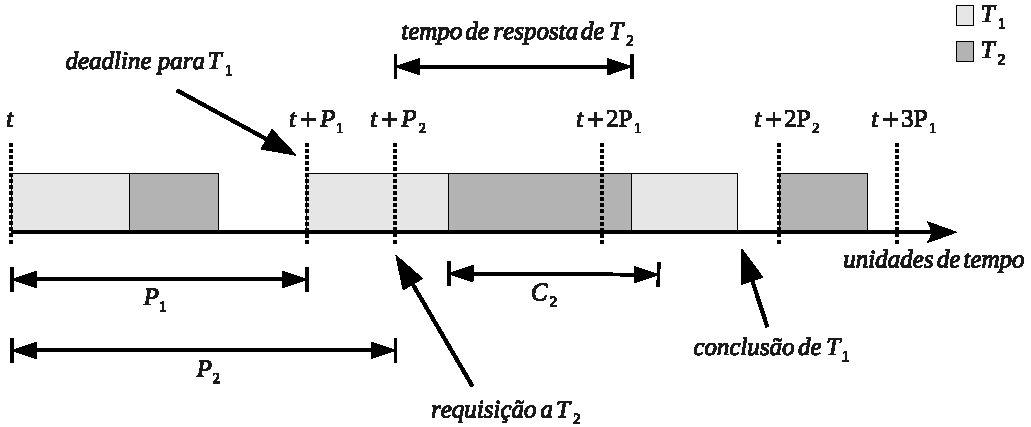
\includegraphics[scale=0.8]{imagens/exemplo-sistema-de-tempo-real.pdf}
        \captionof{figure}{Exemplo do modelo de sistema de tempo real utilizado}
	    \label{fig:exemplo-de-aplicacao}
        \end{center}
        
        Dado o modelo apresentado, é possível definir a \emph{utilização} $U_i$ de uma tarefa $T_i$ em um único processador como sendo $U_i = C_i/P_i$. Diz-se que a \emph{utilização total} por um conjunto de $n$ tarefas $T_i$ é, então, $$U = \sum_{i=1}^{n}\frac{C_i}{P_i}.$$
        
        Pode-se supor que a troca de contexto entre tarefas de uma aplicação dá-se através de uma rotina em software. Obviamente esta rotina também ocupa tempo de processamento no sistema, mas esta faixa de tempo pode ser negligenciada no modelo, pois é possível tratá-la como parte do pior tempo de computação das tarefas em execução.
            
    \subsection{Escalonador de Tempo-Real}
        \label{sec:escalonadores}
    
        Um sistema operacional de tempo real, também chamado de RTOS (\emph{Real-Time Operating System}), é o programa de computador que, além de atender a outras responsabilidades, ordena a execução de tarefas da aplicação de modo a responder em tempo hábil alguma requisição. Mais detalhadamente, o componente do RTOS responsável por esta ordenação é o \emph{escalonador de tempo real} \cite{Li:2003,Pillai:2001}. É este componente que deve prover um ou mais algoritmos que resolvem as prioridades de execução das tarefas do sistema, a fim de que nenhuma delas perca seu deadline.
        
        Para que o escalonador de tempo real seja capaz de garantir a execução em tempo hábil de um conjunto de tarefas, duas condições são estabelecidas:
        
        \begin{itemize}
        	\item O conjunto de tarefas deve ser \emph{escalonável}. Isto significa que o conjunto de tarefas deve passar por um ou mais testes propostos pelo algoritmo do escalonador, justamente para que este conjunto satisfaça as premissas de modo que o algoritmo mantenha suas propriedades. Estes testes são chamados de \emph{testes de escalonabilidade}.
        	\item Nenhuma das tarefas excede seu pior tempo de computação (como elaborado na seção \ref{sec:modelo-de-sistema-de-tempo-real}).
        \end{itemize}
        
        Ainda quanto à ordenação realizada pelo escalonador, esta pode ser entendida como a atribuição de uma prioridade a cada tarefa. Essa atribuição pode ser realizada durante a execução ou previamente. Quando as prioridades são decididas durante execução, diz-se que o escalonador ou o escalonamento é \emph{dinâmico}. No caso em que as prioridades são atribuídas anteriormente à execução, diz-se que o escalonador ou o escalonamento é \emph{estático}.
        
        Quando um escalonador pode interromper a execução de uma tarefa para que uma de maior prioridade ganhe o processador, diz-se que este é um \emph{escalonador preemptivo}.
        
        Dentre os algoritmos para escalonadores de tempo real existentes, este trabalho utiliza o \emph{Earliest Deadline First}, ou simplesmente EDF. Usualmente, diz-se então que o escalonamento ou escalonador utilizado é EDF, e é nele que a heurística \emph{Cycle-conserving RT-DVS} para EDF se baseia. O mecanismo de ordenação do algoritmo EDF é explicado na subseção seguinte (\ref{sec:edf}).
                   
    \subsection{Escalonador \emph{Earliest Deadline First}}
        \label{sec:edf}
        
        O algoritmo \emph{Earliest Deadline First} é um algoritmo para escalonamento dinâmico. Seu funcionamento dá-se com a atribuição de prioridades às tarefas, de modo que quanto mais próxima do deadline a tarefa está, maior é sua prioridade \cite{Liu:1973}. A figura \ref{fig:exemplo-edf} demonstra um exemplo de escalonamento EDF para duas tarefas, onde cada $d_i$ representa deadlines para a tarefa $T_i$. Ambas tarefas tem sua primeira requisição em $t$. Observe que no primeiro deadline $d_1$ acontece a preempção de $T_2$, pois neste momento há uma nova requisição de $T_1$, que por sua vez apresenta um deadline mais próximo que $T_2$.
        
        \begin{center}
    	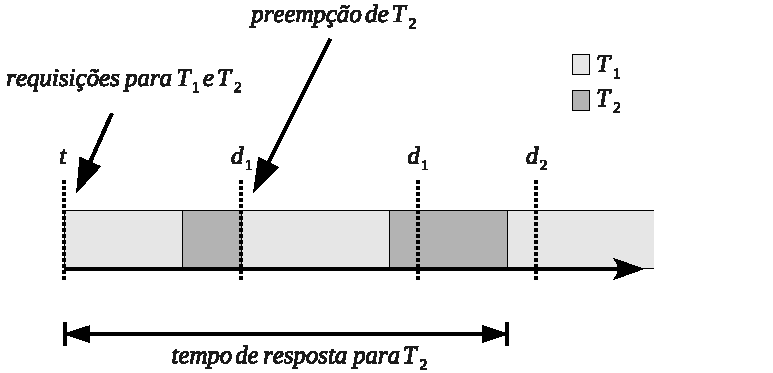
\includegraphics[scale=0.8]{imagens/exemplo-edf.pdf}
        \captionof{figure}{Exemplo de escalonamento EDF para duas tarefas}
	    \label{fig:exemplo-edf}
        \end{center}        
        
        Um teste de escalonabilidade para o EDF é o seguinte:
        
        Dado um conjunto $T$ de $n$ tarefas $T_i$, para $1 \leq i\leq n$, tais que:

   	    \begin{itemize}
	        \item sejam independentes entre si;
	        \item sejam passíveis de preempção;
	        \item sejam periódicas;
	        \item possuam deadlines iguais a seus respectivos períodos.
	    \end{itemize}
        
        Então, $T$ é escalonável por um escalonador EDF se, e somente se $$ \sum_{i=1}^{n} \frac{C_i}{P_i} \leq 1.$$
        
        O teste descrito nada mais é do que a verificação da utilização total do processador para conjunto de tarefas $T$. Este teste, por si só, já é necessário e suficiente para que o conjunto de tarefas seja escalonável.
        
    \section{\emph{Dynamic Voltage and Frequency Scaling}}
    
        \emph{Dynamic Voltage and Frequency Scaling} (DVFS), ou também \emph{Dynamic Voltage Scaling} (DVS), é a capacidade ou atitude de um processador alterar sua tensão e frequência durante a execução de um programa, ou seja, alterar sua tensão e frequência dinamicamente \cite{Pillai:2001}.
        
        A ideia desta técnica é oferecer um contrato entre desempenho de processamento e consumo de energia. A fundamentação desta troca se estabelece sobre duas importantes características da tecnologia de sistemas computacionais atual: \begin{itemize} \item Primeiramente, quase a totalidade destes sistemas são baseados em lógica CMOS. \item Em segundo, o pico de computação das aplicações, sejam elas embarcadas ou não, é usado apenas durante uma pequena fração do tempo de funcionamento desses sistemas. \end{itemize}
        
        % No parágrafo anterior falta uma citação sobre CMOS
        
        A primeira característica apresentada influi no contrato, pois, pelas propriedades físicas dos circuitos CMOS atuais, a energia dissipada ($P$) é fortemente relacionada à frequência ($f$) e à tensão de funcionamento ($V$) do sistema, dois fatores fundamentais para o desempenho \cite{Snowdown:2005}. Esta proporção é visível da seguinte forma: $$P \propto fV^2.$$
        
        Levando em conta que o tempo de computação é inversamente proporcional a $f$, pode-se dizer que a energia $E$, utilizada na computação de uma tarefa em um processador CMOS, é estabelecida conforme a seguinte proporção: $$E \propto V^2.$$ 
        
        Detalhando esta primeira característica, diminuindo a frequência para a redução de consumo de energia, o tempo para o término da dada tarefa aumenta, ou seja, mesmo com um consumo energético menor, este consumo será mantido por mais tempo. Por outro lado, diminuindo-se a frequência, aumenta-se o período entre os chaveamentos do circuito digital, tornando o efeito temporal da capacitância mais tolerável, daí a possibilidade de redução da tensão. Mesmo que o tempo de execução da tarefa seja linearmente proporcional à frequência, a energia gasta é quadraticamente proporcional à tensão, permitindo um ganho energético. Na figura \ref{fig:dvs} um exemplo é ilustrado para uma tarefa que possui tempo de computação exato de 20 milisegundos a 20MHz. Mesmo reduzindo-se pela metade a frequência do processador, tomando-se o dobro de tempo para a execução da tarefa exemplo, ainda há redução no consumo de energia.    

        \begin{figure}
        \begin{center}
        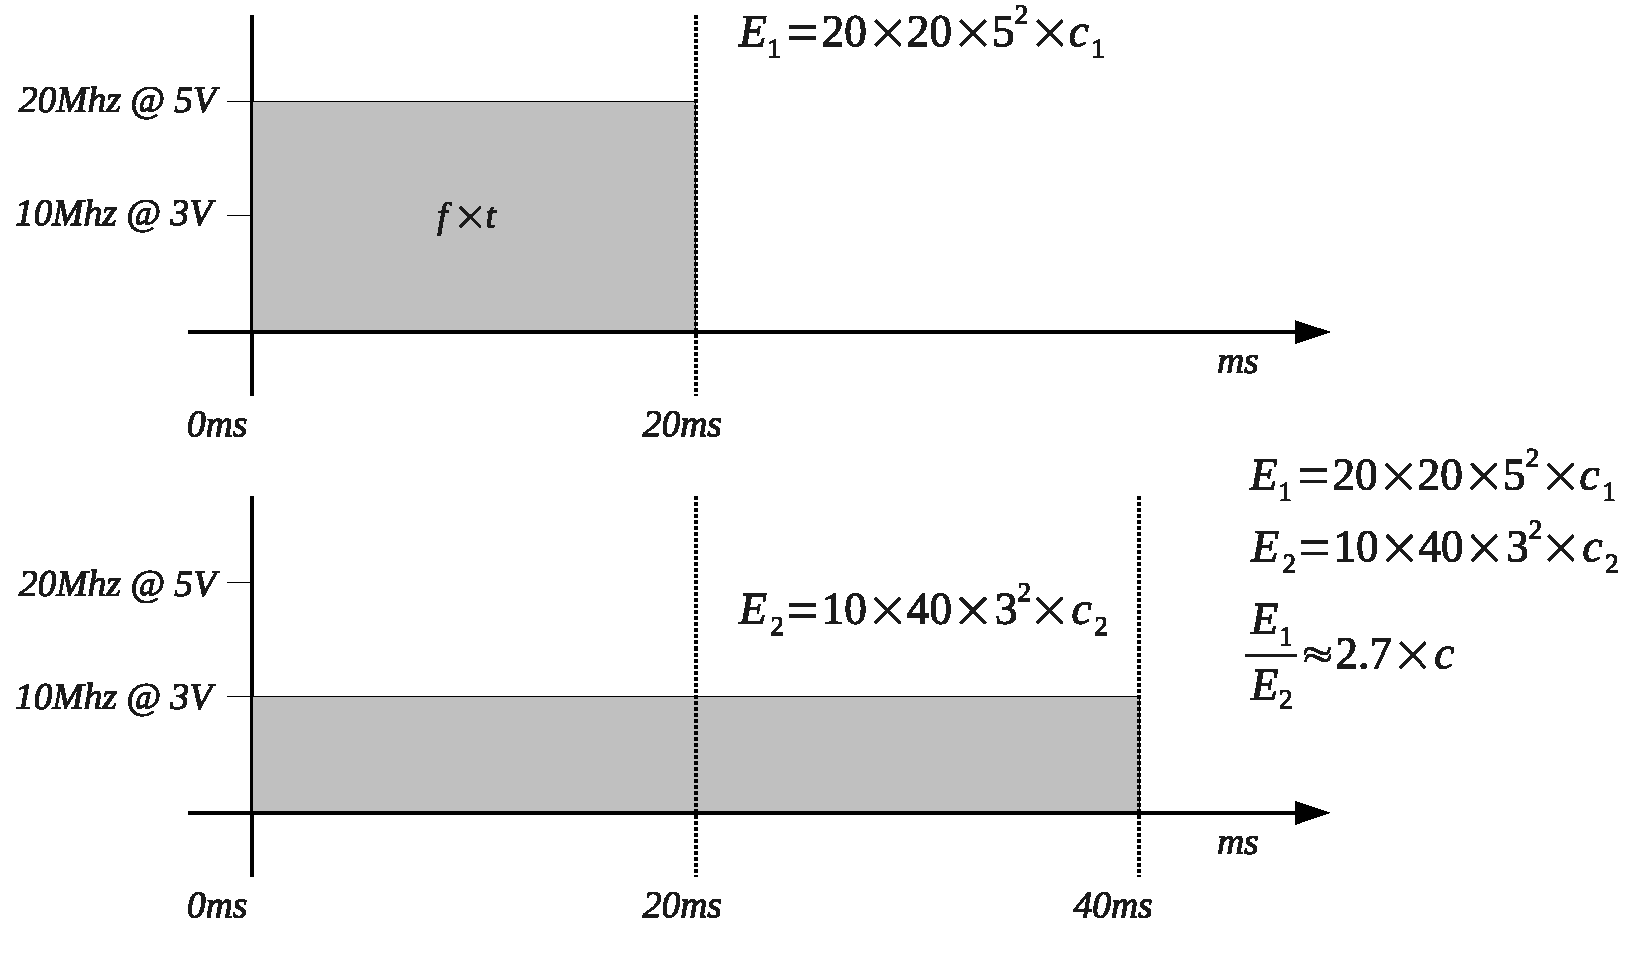
\includegraphics[scale=0.5]{imagens/exemplo-tarefas-dvs.pdf}
        \captionof{figure}{Exemplo de ganho energético obtido através de DVFS}
        \label{fig:dvs}
        \end{center}
        \end{figure}
        
        Finalmente, tendo em foco a segunda característica, que diz respeito ao pico e a média de computação necessária em um sistema computacional, pode-se então, ajustando-se a frequência às necessidades da aplicação, consumir a energia necessária para alto desempenho somente nos momentos realmente requisitados pela aplicação.
        
        Os processadores que implementam esta tecnologia oferecem uma interface que permite, ao software em execução, a alteração dinâmica da tensão. Essa interface, geralmente, é disponível na forma de registradores ou instruções especiais. Um exemplo seria a implementação Intel SpeedStep para núcleos ARM. Neste caso, expande-se a arquitetura ARM do processador através de um co-processador, o qual possui registradores acessíveis através do conjunto de instruções ARM padrão. É possível então, através destes registradores, configurar dinamicamente modos de operação não somente para o núcleo (CPU), mas também para o barramento principal e memória. Cada um destes modos de operação estabelece uma tensão e sua respectiva frequência de funcionamento para estes dispositivos \cite{Snowdown:2005}.
        
    \section{\emph{Real-Time Dynamic Voltage and Frequency Scaling}}
    
        \emph{Real-Time Dynamic Voltage (and Frequency) Scaling}, ou simplesmente RT-DVS, é a qualidade que \citeonline{Pillai:2001} atribuíram aos algoritmos que propuseram. Em um sentido mais amplo, pode-se dizer que RT-DVS, ou RT-DVFS, é capacidade de se alterar a tensão e frequência do processador, para fins de economia de energia, de modo que as tarefas do sistema continuem respondendo em tempo hábil.
        
        Já que nem sempre as tarefas de uma aplicação de tempo real acabam executando como seu pior caso ($C_i$), e a utilização do processador nem sempre é total, é possível usufruir da economia energética oferecida pelas técnicas de DVFS em sistemas de tempo real. Por exemplo, se uma tarefa termina sua execução mais cedo que o esperado, como mostrado na figura \ref{fig:exemplo-tarefas-usando-dvs}, pode-se então utilizar a faixa de tempo não utilizada para que uma próxima tarefa seja executada, mas agora com menor desempenho. Esta técnica também é conhecida como \emph{slack reclamation} \cite{Chen:2007}. Ainda assim, esse tipo de decisão deve ser tomada com cautela, de modo que nenhum prazo seja perdido.
        
        \begin{figure}[h]
        \begin{center}
        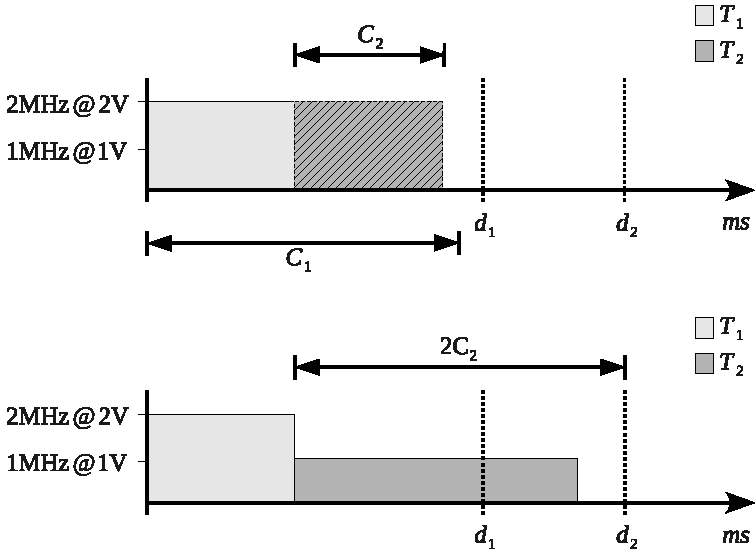
\includegraphics[scale=0.9]{imagens/exemplo-tarefas-usando-dvs.pdf}
        \captionof{figure}{Exemplo de utilização de DVFS em sistemas de tempo real}
        \label{fig:exemplo-tarefas-usando-dvs}
        \end{center}
        \end{figure}
    
    \subsection{Escalonamento em Sistemas RT-DVFS}
        \label{sec:escalonamento-em-sistemas-rt-dvfs}
            
        As primeiras prototipagens de sistemas operacionais embarcados RT-DVFS foram apresentas por \citeonline{Pillai:2001}. Em seu trabalho, foram desenvolvidas heurísticas que, fracamente acopladas ao escalonador do sistema operacional, oferecem consciência energética aos algoritmos \emph{Rate-Monotonic} \cite{Liu:1973} e EDF. \citeonline{Pillai:2001} propõem três classes de heurísticas: as de alteração de tensão estáticas (\emph{Static Voltage Scaling}), as de conservação de ciclos (\emph{Cycle-conserving RT-DVS}) e as de previsão (\emph{Look-ahead RT-DVS}). Das classes citadas, este trabalho utiliza em sua implementação as duas primeiras em conjunto ao algoritmo de escalonamento EDF. Esta escolha é justificada pela simplicidade de implementação e, ao mesmo tempo, por permitir a comparação entre heurísticas que tomam decisões estaticamente e heurísticas que tomam decisões durante a execução do sistema. O funcionamento das duas heurísticas escolhidas é explicado nas seções seguintes.
            
    \subsection{\emph{Static Voltage Scaling} para EDF}
        \label{sec:estaticos}
    
        A primeira abordagem de \citeonline{Pillai:2001} é um mecanismo simples que se beneficia da alteração de tensão e frequência, mantendo a execução das tarefas dentro de seus respectivos prazos. Como o próprio nome da técnica sugere, esta é uma configuração estática da frequência do processador (não se deve confundir com escalonamento estático, como apresentado na seção \ref{sec:escalonadores}). A ideia é obter a menor frequência possível de modo que, mesmo neste baixo desempenho, o conjunto de tarefas satisfaça o teste de escalonabilidade do escalonador EDF. A frequência, por ser configurada estaticamente, só é alterada se o conjunto de tarefas é alterado. Assim sendo, se durante a execução, uma nova tarefa é adicionada ao sistema, o conjunto de tarefas está sendo alterado, então é necessária novamente a escolha de uma nova frequência de funcionamento.
        
        É possível perceber que, alterando a frequência de operação por um fator $\alpha$ $(0 < \alpha \leq 1)$, será necessário alterar os piores tempos de computação para cada tarefa em um fator $1/\alpha$. Observe que os períodos e deadlines, seguindo o modelo apresentando na seção \ref{sec:modelo-de-sistema-de-tempo-real}, mantêm-se inalterados. Com um novo pior tempo de computação, haverá alteração no teste de escalonamento.
        
        % Acrescentar uma figura aqui
        
        Para verificar a escalonabilidade dos conjuntos de tarefas, utiliza-se o teste apresentado na seção \ref{sec:edf}. Este teste, agora com a frequência alterada pelo fator $\alpha$, ficaria como o seguinte\footnotemark:
        
        \footnotetext[1]{O novo teste de escalonabilidade nada mais é do que a aplicação do fator $\frac{1}{\alpha}$ a cada $C_i$ na antiga inequação. Multiplicando os dois lados da inequação por $\alpha$, obtém-se a expressão apresentada aqui.}
        
        Dado um conjunto $T$ de $n$ tarefas $T_i$, para $1 \leq i\leq n$, tais que:
            
   	    \begin{itemize}
	        \item sejam independentes entre si;
	        \item sejam passíveis de preempção;
	        \item sejam periódicas;
	        \item possuam deadlines iguais a seus respectivos períodos.
	    \end{itemize}
       
        $T$ é escalonável por um escalonador EDF se, e somente se $$ \sum_{i=1}^{n} \frac{C_i}{P_i} \leq \alpha.$$
        
        A consciência energética da heurística \emph{Static Voltage Scaling} para EDF consiste então na otimização do conjunto das $m$ frequências possíveis para o processador, sendo escolhida a menor delas capaz de manter o conjunto de tarefas escalonável segundo o teste apresentado. Assim, escreve-se o procedimento \emph{seleciona-frequência}, como expresso no algoritmo \ref{alg:seleciona-frequencia}.
                
        \begin{algorithm}[H]
        \SetKwFunction{testeEDF}{teste-EDF}
        \SetKwFunction{testeRM}{teste-RM}
        \SetKwFunction{seleciona}{seleciona-frequência}
        \SetKwBlock{bloco}{}{}

        \testeEDF{$\alpha$}:
        \bloco{
           \eSe {$\sum_{i=1}^{n} \frac{C_i}{P_i} \leq \alpha$}
                { \Retorna{verdadeiro} }
           { \Retorna{falso} }
        }

        \seleciona:
        \bloco{
            use a menor frequência $f_i \in \left\{f_1,\ldots,f_m|f_1 < \cdots < f_m\right\}$\\
            tal que \testeEDF{$f_i/f_m$} retorne verdadeiro.
        }

        \label{alg:seleciona-frequencia}
        \caption{Alteração estática de tensão para EDF}
        \end{algorithm}
       
        Se o conjunto de tarefas passa no teste de escalonabilidade para a nova frequência e, ainda, as tarefas também não ultrapassam seu novo pior caso de resposta, este mecanismo assegura que os deadlines não serão comprometidos. Se o teste de escalonabilidade falha para todas configurações possíveis, então não é possível escalonar o conjunto de tarefas.
        
        Pela seleção da frequência ser realizada anteriormente à execução do conjunto de tarefas, o novo algoritmo torna-se fracamente acoplado ao escalonador de tempo real \cite{Pillai:2001}, ou seja, uma prévia configuração do sistema pode ser feita, então um escalonador EDF comum pode realizar seu trabalho normalmente, sem necessidade desta entidade entrar em contato com a heurística. Por outro lado, este mecanismo não oferece economia de energia nos momentos onde uma tarefa não atinge seu pior tempo de computação, o que pode acontecer em sistemas reais. Para este caso, algoritmos que levam em conta a utilização real da tarefa, como os expostos adiante, conseguem um melhor benefício.
        
        Um exemplo, apresentado na figura \ref{fig:escalonamento-estatico}, pode ser realizado com as tarefas mostradas na tabela \ref{tab:tarefas-exemplo}. Observe que o pior tempo de resposta ($C_i$) está avaliado para a máxima frequência de funcionamento do processador, ou seja, o caso onde $\alpha=1$ (cenário \emph{a} na imagem). Em um conjunto de três configurações possíveis para frequência, a correspondente a $\alpha=0,75$ é a menor delas que ainda mantém o conjunto de tarefas escalonável (cenário \emph{b} na imagem). Para $0,75>\alpha>0$, algumas tarefas podem perder seus prazos de execução, como é o caso no cenário \emph{c} apresentado na figura, onde a tarefa $T_2$ perde seu deadline.
        
        \begin{figure}[h]
    	\centering
	    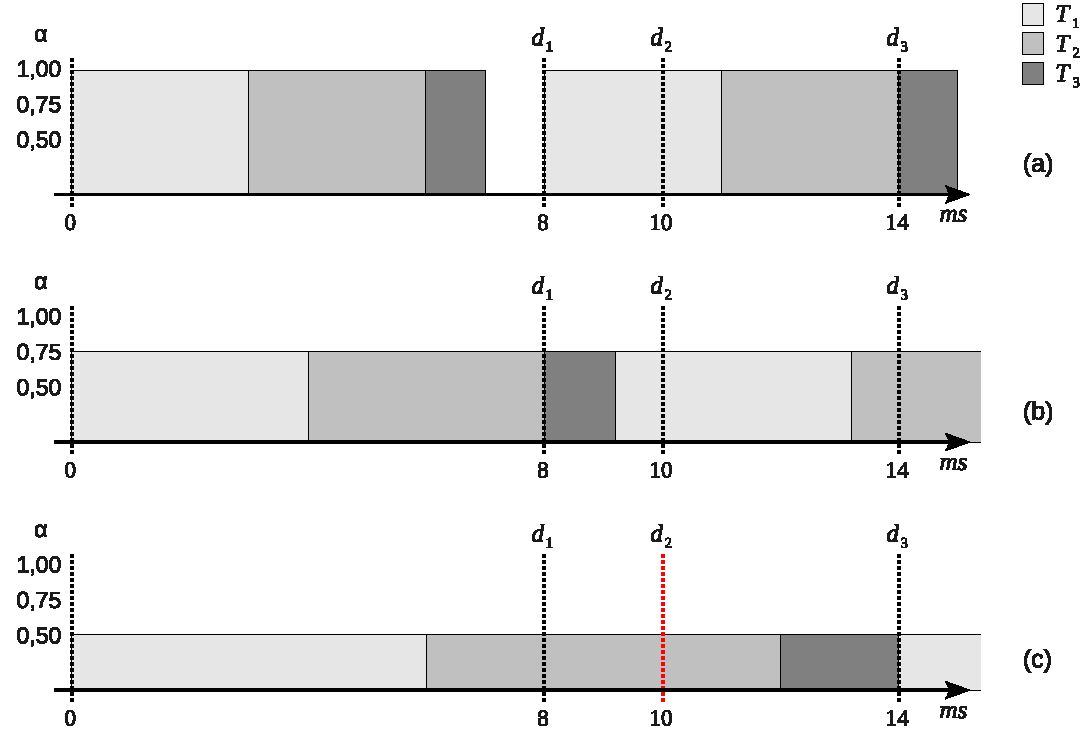
\includegraphics[scale=0.8]{imagens/exemplo-svs-edf.pdf}
    	\caption{Exemplo de escalonamento EDF com alteração estática de frequência}
	    \label{fig:escalonamento-estatico}
        \end{figure}

        \begin{center}
        \begin{table}[h]
        \begin{tabularx}{\textwidth}{ |C|C|C|C| }
            \hline
            Tarefa ($T_i$) &
            Pior Tempo de Computação ($C_i$) &
            Período ($P_i$) &
            Utilização da tarefa ($U_i$)\\ \hline \hline
            
            $T_1$ & $3ms$ & $8ms$ & $0,375$ \\ \hline
            $T_2$ & $3ms$ & $10ms$ & $0,300$ \\ \hline
            $T_3$ & $1ms$ & $14ms$ & $0,071$ \\ \hline
        \end{tabularx}
        \captionof{table}{Exemplo de conjunto de tarefas}
        \label{tab:tarefas-exemplo}
        \end{table}
        \end{center}

        \subsection{\emph{Cycle-conserving RT-DVS} para EDF}
            \label{sec:ccedf}
       
        Uma maneira de tirar maior proveito do uso de DVFS durante o escalonamento EDF é aproveitar as folgas de tempo obtidas quando tarefas não atingem seu pior tempo de computação. De qualquer modo, quando uma tarefa é requisitada para sua execução, não é possível prever o tempo de computação real que será utilizado. Uma solução, proposta por \citeonline{Pillai:2001}, está em assumir que a tarefa inicialmente ocupa seu pior tempo de resposta, mas ao seu término, verificar qual foi o real uso do processador na execução. A ideia desta heurística é então, utilizando estes dados capturados durante a execução das tarefas, adequar o desempenho do processador próximo à utilização real que o conjunto de tarefas promove.
       
        Na heurística \emph{Cycle-conserving RT-DVS} para EDF, três eventos do sistema devem ser capturados: a alteração do conjunto de tarefas, o início da execução de uma tarefa e a conclusão de uma tarefa. A estes eventos, ações são atribuídas:
                      
        \begin{description}
            \item[Na alteração do conjunto] de tarefas, é possível comportar-se como na heurística estática apresentada anteriormente, ou seja, aplicar o algoritmo \ref{alg:seleciona-frequencia} apresentado anteriormente. Isto garante configuração inicial válida para o sistema, sem nenhum prejuízo, já que a heurística \emph{Static Voltage Scaling} é baseada em um cenário de pior caso.
        	\item[No início da execução] da tarefa $T_i$, calcula-se sua utilização no pior caso de computação. Ou seja, assume-se $U_i=C_i/P_i$ até a conclusão da tarefa. Por final, calcula-se a utilização total e aplica-se o algoritmo \ref{alg:seleciona-frequencia} para a seleção da configuração desejada.
        	\item[Na conclusão] da tarefa $T_i$, calcula-se também sua utilização, mas baseando-se agora em seu tempo de computação real $cc_i$. Ou seja, assume-se $U_i=cc_i/P_i$ até que haja uma nova requisição para a tarefa. Novamente, com a utilização calculada, aplica-se o algoritmo \ref{alg:seleciona-frequencia} para a seleção da configuração desejada.
        \end{description}
        
        % Conferir esse exemplo: ver se a tabela de invocações corresponde à execução com alpha = 1.
        
        A figura \ref{fig:cc-edf} demonstra a heurística \emph{Cycle-conserving RT-DVS} para EDF sendo aplicada. O conjunto de tarefas da tabela \ref{tab:tarefas-exemplo} é utilizado como exemplo. A tabela \ref{tab:invocacoes} mostra o tempo de resposta destas tarefas com $\alpha=1$, para a primeira e segunda invocação de cada tarefa. As setas apontam a utilização total calculada no início da execução da tarefa (utilizando-se dados estáticos), e também a utilização total calculada com os dados obtidos \textit{online}, ao final da execução das tarefas.
        
        \begin{figure}[ht]
    	\centering
	    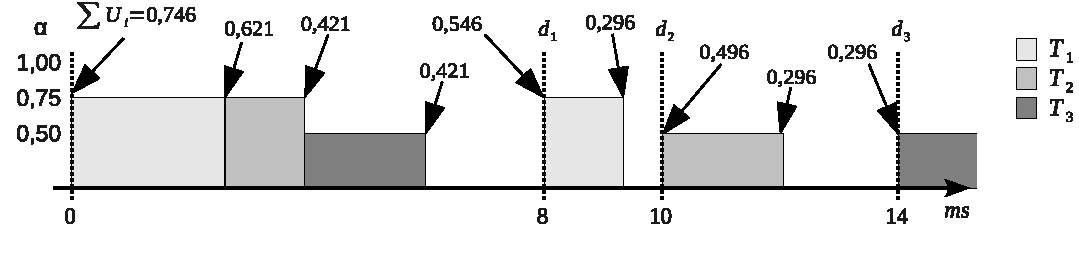
\includegraphics[scale=0.8]{imagens/exemplo-cc-edf.pdf}
    	\caption{Exemplo de escalonamento \emph{Cycle-conserving RT-DVS} para EDF com a utilização calculada em cada início e término de tarefa}
	    \label{fig:cc-edf}
        \end{figure}
        
        \begin{center}
        \begin{table}[ht]
        \begin{tabularx}{\textwidth}{ |C|C|C| }
            \hline
            Tarefa &
            Tempo de Computação na Primeira Invocação &
            Tempo de Computação na Segunda Invocação \\ \hline \hline
            
            $T_1$ & 2$ms$ & 1$ms$ \\ \hline
            $T_2$ & 1$ms$ & 1$ms$ \\ \hline
            $T_3$ & 1$ms$ & 1$ms$ \\ \hline

        \end{tabularx}
        \captionof{table}{Tempo de computação para cada invocação do exemplo}
        \label{tab:invocacoes}
        \end{table}
        \end{center}        
        
        O algoritmo \ref{alg:cc-edf} representa o comportamento da heurística \emph{Cycle-conserving RT-DVS} para EDF. Os procedimentos \emph{tarefa-requisitada} e \emph{tarefa-concluída} são executados em seus respectivos eventos para uma dada tarefa $T_i$. A cada alteração do conjunto de tarefas, \emph{seleciona-frequência} (algoritmo \ref{alg:seleciona-frequencia}) é chamado. Observe que este algoritmo necessita do dado $cc_i$, que é o tempo de computação real utilizado pela tarefa $T_i$. Este é um dado que deve ser calculado em tempo de execução pelo sistema operacional, e além disso, disponibilizado na interface de programação oferecida para a implementação das heurísticas.
        
        \begin{algorithm}[H]
        \SetKwFunction{tarefarequisitada}{tarefa-requisitada}
        \SetKwFunction{tarefaterminada}{tarefa-concluída}
        \SetKwFunction{seleciona}{seleciona-frequência}
        \SetKwBlock{bloco}{}{}

        \seleciona:
        \bloco{
            use a menor frequência $f_i \in \left\{f_1,\ldots,f_m|f_1 < \cdots < f_m\right\}$\\
            tal que $U_1+\cdots+U_n \leq f_i/f_m$.
        }
        
        \tarefarequisitada{$T_i$}:
        \bloco{
           $U_i \leftarrow C_i/P_i$\\
           \seleciona
        }
           
        \tarefaterminada{$T_i$}:
        \bloco{
           $U_i \leftarrow cc_i/P_i$\\
           \seleciona
        }

        \label{alg:cc-edf}
        \caption{\emph{Cycle-conserving RT-DVS} para escalonador EDF}
        \end{algorithm}     
       
       


    \chapter{Desenvolvimento}
    \label{chap:desenvolvimento}
    
    % implementação do porte
        % apresentação  da plataforma de hardware
        % EPOS, mediadores e abstrações
        % programação
        % depuração
    % implementação RT-DVS
    
    Este capítulo apresenta o desenvolvimento deste trabalho em duas seções. A primeira diz respeito ao porte do sistema operacional, apresentando o estudo de caso EPOS e suas características necessárias ao entendimento do capítulo, além da descrição da plataforma de hardware alvo escolhida. A segunda seção trata da criação de suporte a RT-DVFS sobre o sistema operacional EPOS já portado para a plataforma alvo.
    
    \begin{comment}
    \section{Porte do Sistema Operacional}
        \subsection{EPOS e Portabilidade}
            % Overview do que é o EPOS
            % Conceito de mediadores
            % Conceito de abstrações
        
        \subsection{Plataforma Alvo}
            \subsubsection{Programação}
            \subsubsection{Depuração}
            \subsubsection{Suporte a DVFS}

        \subsection{Run-time C++}
        \subsection{Inicialização do EPOS}
        \subsection{Implementação de Mediadores}
        \subsection{Mediador de Máquina e DVFS}
        
    \section{Criação do Ambiente RT-DVFS}
    \end{comment}
            
    \section{Porte do Sistema Operacional}
        \label{sec:plataforma}
        
        Esta seção apresenta a avaliação de uso da plataforma Gumstix Connex \cite{gumstix-legacy}, que possui um processador Intel PXA255 \cite{pxa255-developers-manual}, com a arquitetura Intel XScale, vastamente utilizada em estudos de energia na última década \cite{Chen:2007}. Além disso, também é descrita a estruturação do sistema EPOS necessária para o desenvolvimento do porte para a plataforma de hardware citada.
        
        \subsection{EPOS e Portabilidade}
        
        O EPOS (\emph{Embedded Parallel Operating System}) \cite{Frohlich:2001} é um sistema operacional direcionado a aplicações embarcadas de alto desempenho. Segue a metodologia ADESD (\emph{Application-Driven Embedded System Design}), utilizando técnicas de orientação a aspectos e programação estática em busca de se adequar às restrições presentes nas aplicações para o qual é utilizado.
        
        Ao mesmo tempo que o EPOS busca a especialização para a aplicação, deve lidar com a gama de plataformas utilizadas para a produção e durante o ciclo de vida das aplicações. O sistema operacional hoje, conta com portes para diversas plataformas, como IA32, ARM7, AVR8, MIPS e PowerPC. Seguindo a metodologia ADESD, ou seja, sendo um sistema orientado a aplicação, a troca da plataforma a ser utilizada na aplicação deve permanecer transparente ao programador do sistema.
        
        O EPOS busca balanço entre desempenho e portabilidade através de dois artefatos: primeiro, rotinas de pré-configuração, presentes no sistema como a entidade \emph{Setup Utility}; em segundo, os mediadores de hardware.
        
        \subsubsection{\emph{Setup Utility}}
            \label{sec:setup-utility}
        
        As rotinas de pré-configuração do sistema são porções de código dependentes de hardware. Elas são executadas anteriormente ao ambiente do sistema operacional. Seu papel é construir o contexto fundamental para a execução do EPOS. Isto significa oferecer um cenário seguro de execução e inicialização do sistema, garantido, por exemplo, a existência de uma pilha consistente ou o desligamento de interrupções. Estas rotinas facilitam a portabilidade devido ao fato de reduzirem a complexidade de outros componentes do sistema operacional.
        
        Ao final da execução do componente \emph{Setup Utility}, o controle do sistema é entregue ao suporte dinâmico (\emph{run-time}) da linguagem C++ (linguagem na qual maior parte do sistema é escrita), que desencadeia a inicialização dos outros componentes do EPOS.
        
        \subsubsection{Mediadores de Hardware}
        
        Os mediadores de hardware do EPOS oferecem interfaces simples para acesso a itens dependentes de máquina. Assim, componentes mais abstratos do sistema (chamados de \emph{abstrações}), como por exemplo, \emph{Thread} ou \emph{Scheduler}, podem permanecer com suas implementações portáveis independentemente da plataforma alvo.
        
        % Apresentados estes artefatos, conclui-se que, para a criação de um novo porte do sistema EPOS, basta implementar as rotinas de pré-configuração e os mediadores de hardware necessários aos componentes de mais alto-nível utilizados.

        \subsection{Plataforma Alvo}
            \label{sec:plataforma-alvo}
        
            A plataforma Connex faz parte de uma linha descontinuada de placa-mães da companhia Gumstix. Esta placa possui um processador Intel PXA255 com microarquitetura Intel XScale. O PXA255 mostrou-se interessante para os fins deste trabalho, pois o núcleo Intel XScale é justamente direcionado para aplicações embarcadas que exijam alta performance e baixo consumo de energia \cite{pxa255-developers-manual}.
            
            % Acrescentar uma figura da arquitetura interna de barramento/CPU/memória.
            
            O processador PXA255 suporta DVFS para três componentes do processador: a CPU, o barramento principal e memória \cite{Snowdown:2005}, fator fundamental para o desenvolvimento deste trabalho. Além disso:
            
            \begin{itemize}
                \item O laboratório onde este trabalho foi desenvolvido possui um conjunto de placas Connex e outros módulos de expansão.
                \item Mesmo com o processador PXA255 oferecendo uma interface JTAG \cite{jtag-standard} para depuração, as placas da linha Connex não oferecem acesso necessário a este recurso. Por outro lado, estas placas Gummstix podem ser emuladas através do QEMU \cite{qemu-website}. Felizmente, o QEMU possui opções de depuração junto ao GDB \cite{gdb-website}, de modo que seja possível a supervisão da execução de instruções passo a passo na plataforma.
                \item Processadores compatíveis com o PXA255 e sua arquitetura já estão bem estabelecidos na comunidade de sistemas embarcados e RT-DVFS. Muitos trabalhos exibem experimentos utilizando a plataforma \cite{Chen:2007}. Mesmo que a linha Connex tenha sido descontinuada no ano de 2009 pela Gumstix, ainda assim, versões recentes de placa-mães do mesmo fabricante utilizam arquiteturas compatíveis com a Intel XScale \cite{gumstix-products}. Assim sendo, além de um cenário de estudo presente em outras publicações, o projeto EPOS também se beneficia, já que o sistema será portado para uma plataforma que é amplamente utilizada em aplicações embarcadas que necessitam de baixo consumo de energia e alto desempenho.
                \item A arquitetura Intel XScale utiliza o conjunto de instruções ARMv5TE, mantendo compatibilidade binária com o conjunto ARMv4T \cite{arm-arm}. Felizmente o EPOS já possui porte para plataformas ARM7, sendo que estas seguem a arquitetura ARMv4T. Assim, é possível herdar parte considerável do suporte de baixo nível necessário ao EPOS e também reaproveitar a implementação de alguns componentes, como o mediador de CPU, responsável, por exemplo, pelas rotinas de troca de contexto.
            \end{itemize}
            
            A Gumstix Connex foi escolhida como plataforma de implementação deste trabalho, não somente por oferecer o suporte a DVFS, mas também pelos fatores facilitadores de implementação, além de benefícios experimentais ao EPOS.
                
        \subsection{Programação da Plataforma}
            \label{sec:programacao}
        
        Os primeiros passos tomados para portar o sistema operacional EPOS foram na direção da programação da plataforma Connex. Ela possui 64MB de RAM e uma memória \emph{flash} programável de 128kB, onde o processador busca, em seu endereço base, a primeira instrução para inicialização do sistema.
      
        De qualquer modo, esta memória programável já vem, desde a fabricação da plataforma, tomada pelo U-Boot, um \emph{bootloader} que facilita a inicialização de sistemas operacionais na plataforma. É necessário citar que o U-Boot possui rotinas que auxiliam na programação do sistema, como escrita em memória RAM ou própria \emph{flash}, sendo possível até carregar imagens executáveis utilizando o protocolo Kermit, isto através da porta serial disponível em uma das placas de expansão da plataforma Connex.
        
        Como a placa Connex não oferece acesso à interface JTAG oferecida pelo PXA255, a qual facilitaria a escrita da \emph{flash}, a melhor alternativa para programação da plataforma foi a utilização do próprio U-Boot. A partir da imagem de memória resultante da compilação do EPOS, que contém o sistema operacional, pode-se criar uma outra compatível com a rotina inicializadora de imagens do \emph{bootloader}. Para tanto, usa-se a ferramenta \emph{mkimage}. Criando a imagem EPOS compatível com o U-Boot, basta carregá-la em memória, utilizando a porta serial através do protocolo Kermit implemetado pelo U-Boot.
        
        \subsection{Depuração}
        
        Confirmado o método de programação da plataforma, procurou-se então testar as facilidades de depuração oferecidas pelo QEMU versão \emph{0.12.5}.
        
        O QEMU necessita de que uma imagem da memória programável seja especificada, logicamente para que a plataforma emulada seja inicializada conforme os moldes da seção anterior (\ref{sec:programacao}). Para que a emulação seja a mais fiel possível à plataforma disponível no laboratório, esta imagem foi criada com a versão \emph{1.2.0} do U-Boot, a mesma presente na placa Connex utilizada para desenvolvimento.
        
        A facilidade ofertada pelo QEMU é colocar-se como monitor remoto do GDB. Assim, é possível conectar o GDB (utilizando TCP) ao QEMU, e supervisionar a execução passo a passo de instruções na plataforma emulada. Até a programação pode ser feita através do GDB, escrevendo a imagem EPOS inicializável na memória emulada, e então, delegando ao U-Boot a inicialização do EPOS.
        
        Com os processos de programação da plataforma e depuração, o suporte técnico necessário para construção do novo porte é concluída.
        
        \subsection{\emph{Setup Utility} e \emph{Run-time C++}}
            \label{sec:setup-e-run-time}

         Para os fins deste projeto, o EPOS é configurado para uso em modo \emph{library}. Isto significa que ele é ligado à aplicação como uma biblioteca estática. Sendo assim, por exemplo, não há a necessidade do uso de chamadas de sistema (usualmente nomeadas \emph{System Calls}) \cite{Frohlich:2001}. 
         
         Para a inicialização do sistema operacional, basta indicar ao U-Boot o endereço da primeira instrução contida na imagem do EPOS. Em seu fluxo normal de inicialização, fluxo \emph{a} na figura \ref{fig:inicializacao-do-EPOS}, \emph{Setup Utility} é o primeiro componente do sistema a entrar em ação. No presente trabalho, pelos motivos apontados a seguir, elimina-se o componente \emph{Setup Utility}, seguindo o fluxo \emph{b} apresentado na figura \ref{fig:inicializacao-do-EPOS}.

        \begin{figure}[h]
        \centering
        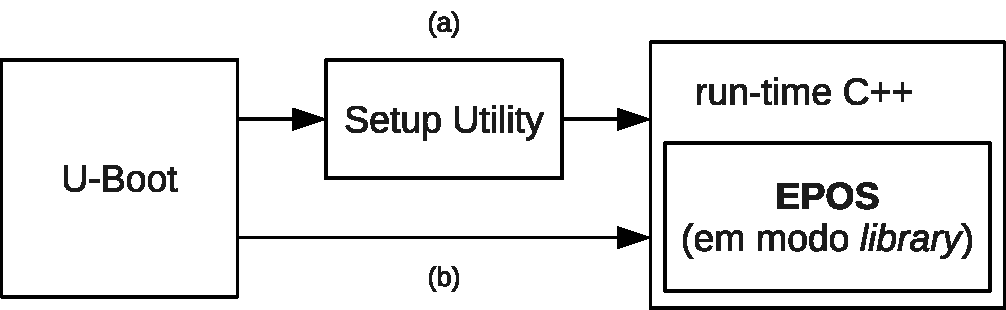
\includegraphics[scale=0.6]{imagens/inicializacao-do-EPOS.pdf}
        \captionof{figure}{Sequência de inicialização do EPOS}
        \label{fig:inicializacao-do-EPOS}
        \end{figure}
        
         Observe que a mesma abordagem é utilizada em outros portes, como por exemplo os para máquinas com arquitetura AVR8, que possuem também uma baixa complexidade relativa.
         
         \subsubsection{Remoção do \emph{Setup Utility}}
         
         Como explicado anteriormente em \ref{sec:setup-utility}, o EPOS possui uma rotina de pré-configuração do hardware. O objetivo dessa rotina é reduzir a complexidade de alguns componentes mais abstratos do sistema operacional. Se comparada a outras plataformas para quais o EPOS foi portado, como IA32 ou PowerPC, o processador PXA255 possui uma complexidade relativamente reduzida, justificando a não necessidade da criação do componente \emph{Setup Utility} para este porte. 
         
         As atividades de pré-configurações reconhecidas como necessárias, para a execução segura do EPOS, foram: o estabelecimento de uma pilha única consistente e o remapeamento dos vetores de interrupção do processador. Para reduzir o tempo de desenvolvimento, estas duas atividades foram delegadas, respectivamente, ao suporte dinâmico da linguagem C++ e às rotinas de inicialização dos mediadores de hardware. O funcionamento destes mecanismos são explicados em subseções seguintes.
         
         \subsubsection{\emph{Run-time} C++}
            \label{sec:run-time-c++}
         
        O \emph{run-time} C++ necessário é responsável por um fator essencial do sistema: inicialização de componentes do sistema, como mediadores ou entidades mais abstratas.
         
        Algumas instâncias de componentes do sistema são tratados pela linguagem como objetos de escopo global, isto faz com que as suas inicializações sejam dependentes da implementação dos mecanismos dinâmicos da linguagem C++ \cite{Stroustrup:1997}. Em outras palavras, isto significa que deve haver a implementação em software do suporte para que estes componentes tenham suas rotinas de inicialização, que foram geradas pelo compilador C++, chamadas antes da execução da função inicial da aplicação.
        
        Este suporte de baixo-nível deve ser escrito em linguagem \emph{assembly}, e portanto é dependente de arquitetura. Felizmente, como foram realizados trabalhos anteriores com processadores de arquitetura ARMv4T, aproveitou-se a compatibilidade binária, pois ARMv4T é um subconjunto das instruções ARMv5TE \cite{arm-arm}, utilizadas na arquitetura Intel XScale.
        
        Aproveitou-se o \emph{run-time} C++ para se adicionar as rotinas responsáveis pela manutenção da pilha do sistema. A arquitetura ARM possui um comportamento indefinido para acessos desalinhados à memória principal. Garantiu-se então, na inicialização da pilha, um endereço alinhado para a mesma. O código gerado pelo compilador faz a manutenção desta propriedade.
        
        Além disso, na arquitetura ARMv5TE, o processador possui pilhas diferenciadas para diversos modos de funcionamento. Isto significa que a pilha utilizada no tratamento de interrupções é diferente da pilha utilizada pela aplicação. Como o EPOS é utilizado em modo \emph{library} neste trabalho, a aplicação e o tratador de interrupções dividem o mesmo espaço de memória, ou seja, devem ser executados em um único modo de operação do processador, com uma única pilha. Como isso não é possível pelo funcionamento padrão da arquitetura, uma adaptação técnica foi realizada no \emph{run-time} C++ para que a existência de uma única pilha fosse transparente ao sistema EPOS.
        
        \subsection{Implementação de Mediadores}
            \label{sec:implementacao-de-mediadores}
        
        Os mediadores do EPOS são a interface para a acesso de componentes da plataforma de hardware \cite{Frohlich:2001}. Assim como as rotinas de pré-configuração, cada mediador é um componente do sistema dependente de máquina. De fato, a implementação dos mediadores para a plataforma PXA255 é o passo final e fundamental para a criação do porte.
        
        Para os fins deste trabalho, não necessariamente todos os mediadores do sistema precisam ser implementados. Isso acontece porque as abstrações que serão utilizadas para experimento estão restringidas a componentes de processo e tempo. Não é preciso, por exemplo, que se implemente mediadores para a interface \emph{bluetooth}, pois sincronizadores, escalonadores, etc. não utilizam este tipo de mediador.
        
        \begin{figure}[h]
        \centering
        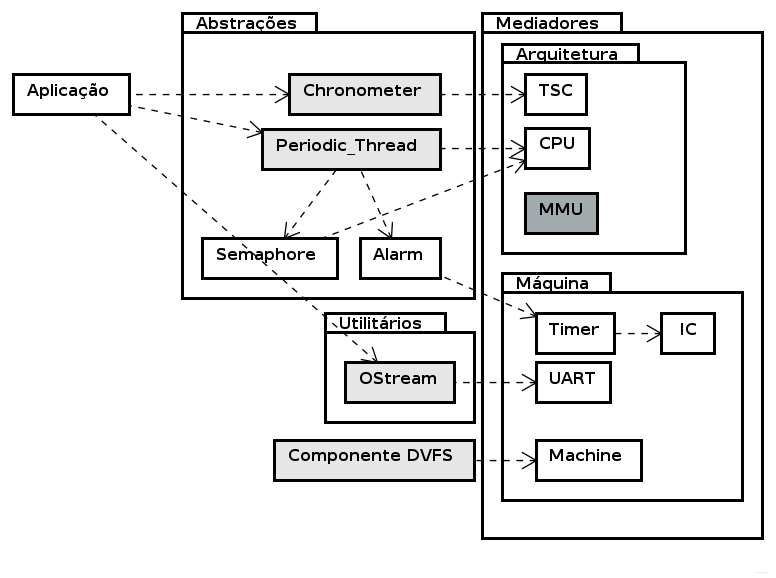
\includegraphics[scale=0.6]{imagens/dependencias-de-mediadores.png}
        \captionof{figure}{Análise de dependências entre aplicação, abstrações e mediadores para o porte}
        \label{fig:dependencias}
        \end{figure}
        
        Em uma análise para definir os mediadores necessários, o diagrama de classes apresentado na figura \ref{fig:dependencias} foi desenvolvido. A aplicação criada posteriormente para experimentos utiliza diretamente somente duas abstrações: \emph{Periodic\_Thread} (tarefas periódicas) e \emph{Chronometer} (cronômetro virtual), além do utilitário \emph{OStream} (saída de dados). Estas dependências exigem, indiretamente, a implementação dos mediadores: \emph{CPU}, \emph{Timer} (temporizador), \emph{UART}, \emph{TSC} (contador temporizado) e \emph{IC} (controlador de interrupções).
        
        O mediador de \emph{MMU} foi também escolhido para implementação, pois foi delegado a ele o remapeamento dos vetores de interrupção (subseção \ref{sec:setup-e-run-time}), procedimento esclarecido mais adiante.
        
        O mediador \emph{Machine}, ou mediador de máquina, é responsável pelas características presentes no PXA255, mas que excedem o conceito de arquitetura (interface binária) do processador. Logo, as atividades de alteração de tensão e frequência devem ser atribuídas a este mediador.
        
        A seguir, são apresentadas informações breves sobre a implementação de cada um destes mediadores.
        
        \subsubsection{\emph{CPU}}
        
        Este mediador é responsável por características como a troca de contexto, entrada e saída em registradores, habilitação de interrupções, e criação de pilhas para novas \emph{threads} no sistema. Sendo assim, é um mediador intimamente ligado com as questões de gerenciamento de tarefas no EPOS. Boa parte deste mediador pôde ser herdada do suporte às arquiteturas ARM utilizadas em projetos anteriores. Ainda assim, pequenas modificações foram necessárias, pois algumas operações de entrada e saída envolvem coprocessadores específicos da arquitetura Intel XScale.
        
        \subsubsection{\emph{Timer}}
        
        Este mediador é requerido por várias abstrações relacionadas a processos, como por exemplo, escalonadores ativos. Como a abstração \emph{Periodic\_Thread} necessita de invocações periódicas, este mediador necessita de implementação.
        
        \subsubsection{\emph{UART}}
        
        O EPOS utiliza este mediador muito cedo em sua inicialização, de modo que seja possível facilitar a depuração em máquinas reais, onde o uso de emuladores e JTAG pode não ser uma realidade. Utilizando a placa Connex em conjunto com sua expansão HWUART, é possível obter informações do sistema em tempo de execução.
        
        \subsubsection{\emph{TSC}}
        
        O TSC (\emph{Time Stamp Counter}) é um dispositivo que auxilia a medição de tempo em alta resolução.
        
        \subsubsection{\emph{IC}}
        
        A arquitetura ARM necessita de um roteamento de interrupções em alto nível. Este mediador abstrai itens referentes aos indicadores de interrupção da máquina, para a decisão de qual tratador instalado chamar. Este mediador é necessário para o funcionamento ideal, por exemplo, do mediador \emph{Timer}.
        
        \subsubsection{\emph{MMU}}
        
         Por padrão, os processadores ARM (como é o caso do Intel XScale) utilizam um vetor de interrupções que encontra-se no endereço 0 emitido pela CPU. Como na máquina Connex este endereço refere-se à \emph{flash} programável, onde já encontra-se instalado um vetor de interrupções do U-Boot, é preciso que seja configurado, através da MMU presente no PXA255, um remapeamento dos endereços emitidos (virtuais) para novos endereços físicos. Assim, é possível traduzir o endereço padrão do vetor de interrupções (endereço 0), que está em \emph{flash}, para um endereço qualquer em RAM, sendo possível instalar nesta memória um vetor de interrupções apropriado ao EPOS.
         
         A MMU do PXA255 segue a VMSAv5 (\emph{Virtual Memory System Architecture version 5}), como descrita no \emph{Arm Reference Manual} \cite{arm-arm}. Na inicialização do mediador de MMU, foi inserida uma rotina que preenche a tabela de descritores de memória. Esses descritores fazem o remapeamento da faixa inicial de 1MB de memória em \emph{flash}, para a primeira faixa de 1MB em RAM. Assim, sempre que uma interrupção for chamada, o acesso ao endereço virtual 0, onde se encontra o vetor de interrupções do U-Boot, será na realidade um acesso ao endereço real em RAM, onde o vetor de interrupções preenchido pelo EPOS se encontra.

        \subsubsection{\emph{Machine}}
        
        Este mediador refere-se ao PXA255 e seus componentes. É ele que deve possuir a interface para que o modo de operação do processador seja alterado. A seção \ref{sec:suporte-dvfs} explica com mais detalhes a implementação do suporte a DVFS.
        
        \subsection{Implementação do Suporte a DVFS}
            \label{sec:suporte-dvfs}
        
        Como citado na seção \ref{sec:plataforma-alvo}, o PXA255 possui suporte a alteração dinâmica de frequência e tensão para três dispositivos: núcleo do processador, barramento do sistema (\emph{PXBus}) e memória SDRAM. A relação entre os principais componentes do PXA255 pode ser observada na figura \ref{fig:arquitetura-do-pxa}. Na mesma figura, em destaque, encontram-se os dispositivos que suportam DVFS.
        
        \begin{figure}[h]
        \centering
        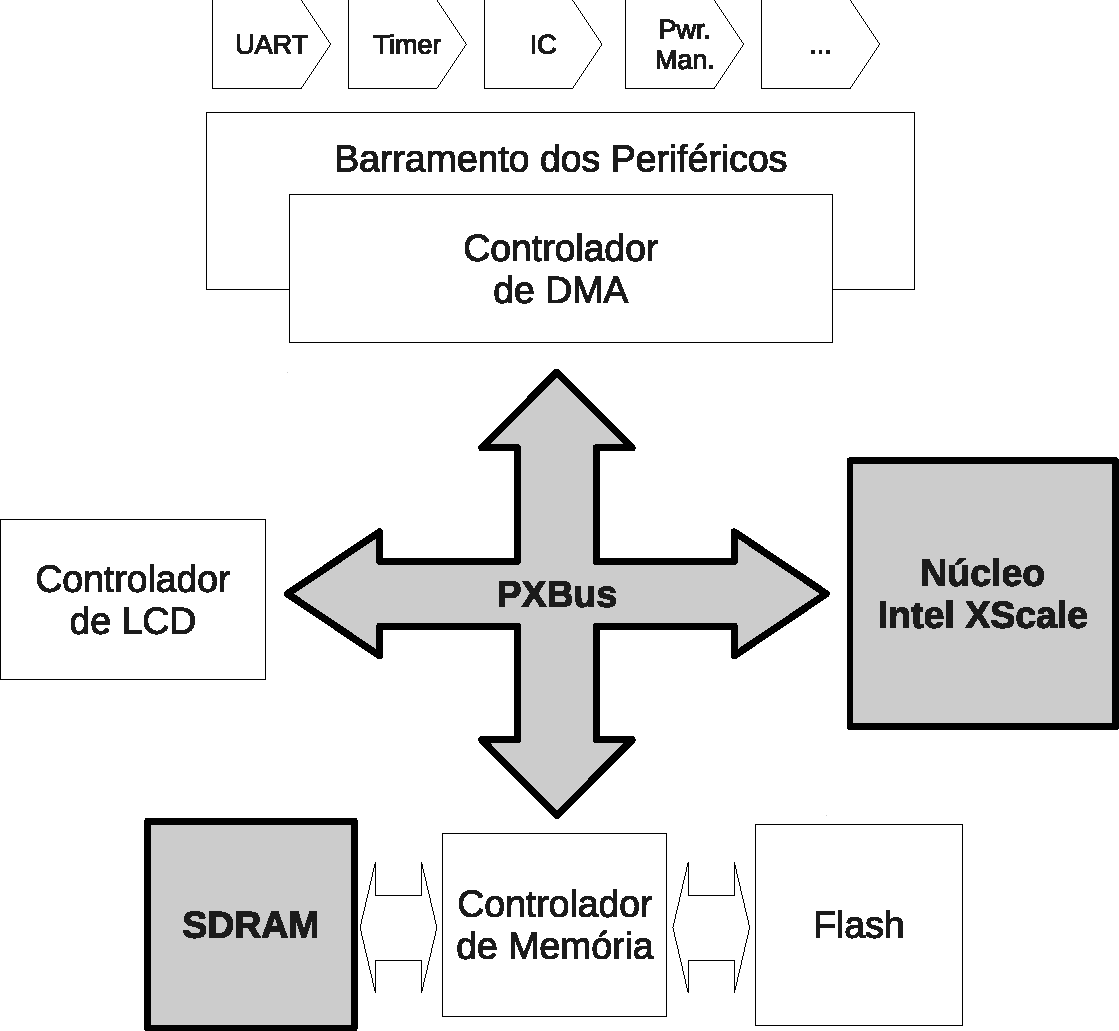
\includegraphics[scale=0.5]{imagens/arquitetura-do-pxa.pdf}
        \captionof{figure}{Representação dos componentes do processador PXA255}
        \label{fig:arquitetura-do-pxa}
        \end{figure}
        
        Segundo o \emph{Intel PXA255 Developer's Manual} \cite{pxa255-developers-manual}, existe um conjunto de configurações de frequência válidas para estes dispositivos. Este conjunto é apresentado na tabela \ref{tab:configuracoes}.
        
        %\begin{center}
        \begin{table}
        \begin{tabularx}{\textwidth}{ |C|C|C|C| }
            \hline
            Tensão do processador ($V$)&
            Frequência do Núcleo ($MHz$)&
            Frequência do PXBus ($MHz$)&
            Frequência da SDRAM ($MHz$)\\ \hline \hline
            1.0 & 99,5 & 50 & 99,5 \\ \hline
            1.0 & 199,1 & 50 & 99,5 \\ \hline
            1.1 & 298,6 & 50 & 99,5 \\ \hline
            1.0 & 132,7 & 66 & 66 \\ \hline
            1.0 & 199,1 & 99,5 & 99,5 \\ \hline
            1.1 & 298,6 & 99,5 & 99,5 \\ \hline
            1.3 & 398,1 & 99,5 & 99,5 \\ \hline
            1.1 & 265,4 & 132,7 & 66 \\ \hline
            1.3 & 331,8 & 165,9 & 83 \\ \hline
            1.3 & 398,1 & 186 & 99,5 \\ \hline
        \end{tabularx}
        \captionof{table}{Possíveis configurações de tensão e frequência para o PXA255}
        \label{tab:configuracoes}
        \end{table}
        %\end{center}
        
        No PXA255, a alteração dinâmica de frequência e tensão é feita através da FCS (\emph{Frequency Change Sequence}). Para qualquer alteração na configuração corrente do processador, invocando a FCS, os seguintes passos devem ser executados diretamente por software \cite{pxa255-developers-manual}:
        
        \begin{enumerate}
            \item Configurar o controlador de memória para que a frequência de atualização da SDRAM seja compatível com as frequências anterior e posterior à FCS.
            \item Desabilitar o controlador de LCD.
            \item Configurar os periféricos para que eles manipulem o atraso que a FCS pode ocasionar no controlador de DMA.
            \item Desabilitar periféricos que não podem acomodar um atraso maior que 500$\mu s$ no tratamento de suas interrupções. Isto se dá porque todas interrupções geradas durante a FCS são tratadas apenas ao final do processo de configuração.
            \item Programar o registrador CCCR (\emph{Core Clock Configuration Register}), de modo a representar uma das configurações apresentadas na tabela \ref{tab:configuracoes}.
            \item Invocar a FCS através da escrita do primeiro bit à direita do registrador CCLKCFG.
        \end{enumerate}
        
        Após a execução do item 6, o fluxo de execução de instruções continua normalmente. Os itens 2, 3 e 4 foram ignorados para a implementação deste porte, pois os controladores de LCD e DMA não foram utilizados em nenhum momento. Além disso, o tratamento de interrupções não foi prejudicado conforme o especificado no item 4.
        
        Para algumas das configurações apresentadas na tabela \ref{tab:configuracoes}, não basta apenas a invocação da FCS pelo registrador CCLKCFG, mas também a invocação do modo \emph{TURBO}, realizada pela escrita do segundo bit à direita do mesmo registrador.
        
        Os métodos para invocação da FCS e do modo TURBO foram encapsulados no mediador de máquina, conforme apresentado no diagrama de classes da figura \ref{fig:mediador-pxa255}.
        
        \begin{figure}[h]
        \centering
        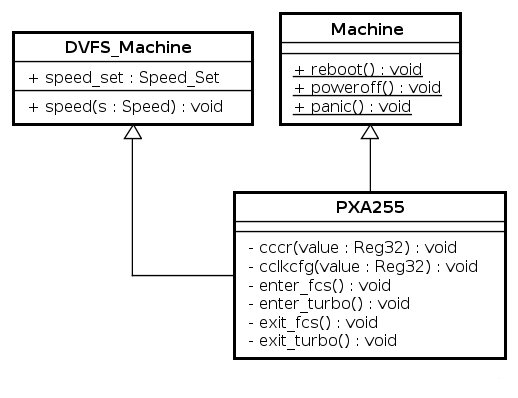
\includegraphics[scale=0.6]{imagens/mediador-pxa255.png}
        \captionof{figure}{Diagrama de classes do mediador de máquina para PXA255}
        \label{fig:mediador-pxa255}
        \end{figure}
        
        Para facilitar a interação entre heurísticas DVFS e o mediador de máquina, uma interface chamada \emph{DVFS\_Machine} foi criada. Essa interface é capaz de fornecer às abstrações do sistema as configurações disponíveis e um meio de aplicá-las. É ela a responsável pelo cumprimento dos passos descritos na enumeração anterior.
           
    \section{Criação do Ambiente RT-DVFS}
        
        Para a adequação com o modelo de sistema de tempo real apresentado na seção \ref{sec:modelo-de-sistema-de-tempo-real}, é utilizada a abstração do EPOS chamada \emph{Periodic\_Thread}. Uma extensão para seu funcionamento foi criada, de modo a captar-se os eventos necessários para a implementação das heurísticas \emph{Cycle-conserving DVS} para EDF e \emph{Static Voltage Scaling} para EDF.

        \subsection{\emph{Threads} Periódicas no EPOS}
            \label{sec:threads-periodicas-no-epos}
        
        A abstração \emph{Periodic\_Thread} do EPOS oferece suporte à execução periódica de tarefas no sistema. A partir dessa abstração, é possível criar um objeto ao qual existem associados um período e uma rotina a ser executada. Este período é representado, na imagem \ref{fig:periodic-thread}, como sendo o atributo \emph{period} da classe \emph{Alarm}. A rotina associada à tarefa periódica é representada na mesma imagem pelo atributo \emph{entry}, herdado por \emph{Periodic\_Thread} da classe \emph{Thread}.
        
        \begin{center}
        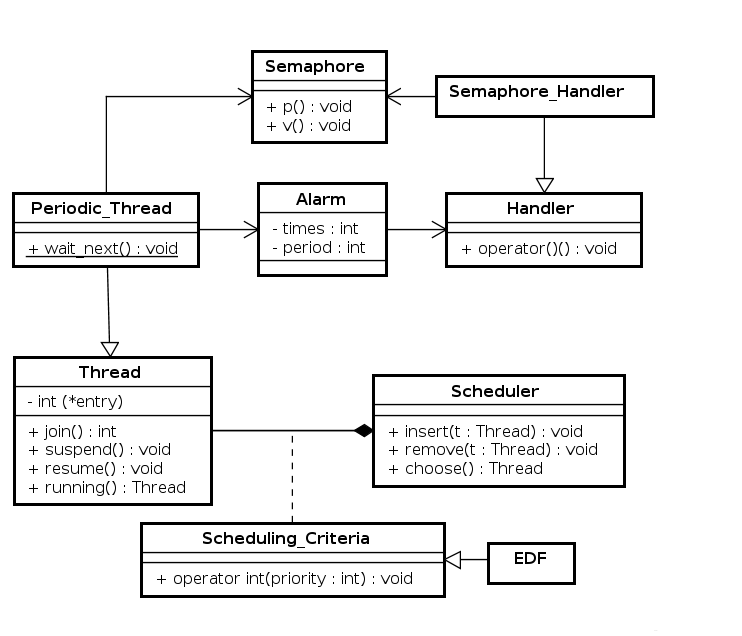
\includegraphics[scale=0.6]{imagens/periodic-thread.png}
        \captionof{figure}{Diagrama de classes apresentando a abstração \emph{Periodic\_Thread}}
        \label{fig:periodic-thread}
        \end{center}
        
        A rotina a ser executada periodicamente deve ser uma função C++ não-membro \cite{Stroustrup:1997}, que deve explicitamente se comportar como um laço, invocando dentro do bloco de repetição a função membro estática \emph{Periodic\_Thread::wait\-\_next}. O exemplo a seguir (\ref{tarefa}) demonstra este artefato para um número \textit{iterations} de repetições da tarefa. Observe que é possível estratificar a execução da tarefa em um ponto para sua inicialização, outro ponto com o corpo de código que será executado repetidamente, e por final, um trecho de código que representa a finalização da tarefa.
        
        
        \begin{lstlisting}[label=tarefa, escapeinside='', float=b, captionpos=b, caption=Exemplo de uma tarefa como uma função não-membro]
        int periodic_task(int iterations){
        
            // inicializa'\textit{çã}'o
            
            for(int i = 0; i < iterations; i++){
                // corpo da tarefa
                Periodic_Thread::wait_next();
            }
            
            // finaliza'\textit{çã}'o
            
            return 0;
        }
        \end{lstlisting}
        
                               
        A \emph{thread} que executa a função membro \emph{Periodic\_Thread::wait\_next}, através da operação ``\emph{p}'' sobre semáforo associado à abstração \emph{Periodic\_Thread}, perde o processador. Esta \emph{thread} entrará em um estado onde ela não ocupará mais a CPU até que a operação ``\emph{v}'' seja realizada sobre o mesmo semáforo. Para oferecer o comportamento periódico às tarefas, a abstração \emph{Alarm} é então utilizada. 
        
        A abstração \emph{Alarm} invoca periodicamente um objeto função (instância da classe \emph{Handler} apresentada na figura \ref{fig:periodic-thread}), neste caso especializado para executar a operação ``\emph{v}'' sobre o semáforo que ``impede'' a repetição do corpo do laço. A \emph{thread} pode então, voltar a ganhar a CPU segundo os critérios do escalonador. Ao recuperar a execução, ela volta ao ponto onde invocou \emph{Periodic\_Thread::wait\_next}, obedecendo ao comportamento do laço escrito.
        
        % Adicionar um diagrama de sequência para este parágrafo.
        
        O escalonador EDF entra como critério de ordenação utilizado pela classe \emph{Scheduler}, também apresentada na figura \ref{fig:periodic-thread}. Para configurar o critério utilizado no escalonamento, o EPOS utiliza o padrão de projeto \emph{traits}, oferecendo a escolha da política como uma configuração estática do sistema \cite{Frohlich:2001}.
        
        \subsection{Modificações no Modelo de \emph{Threads}}
        
        Para implementação das heurísticas para RT-DVFS, algumas modificações foram necessárias no sistema EPOS. Primeiramente, as heurísticas precisam estar cientes de eventos referentes às tarefas, como inicialização, término ou até mesmo alterações no conjunto de tarefas. Ainda, o sistema deve reagir a eventos como a troca de contexto, já que o modelo utilizado é preemptivo. Para que fosse possível atribuir ações a estes eventos, algumas modificações foram necessárias no modelo de \emph{threads} periódicas do EPOS, como apresentado no diagrama de classes da figura \ref{fig:ea-periodic-thread}.
        
        \begin{figure}[h]
        \begin{center}
        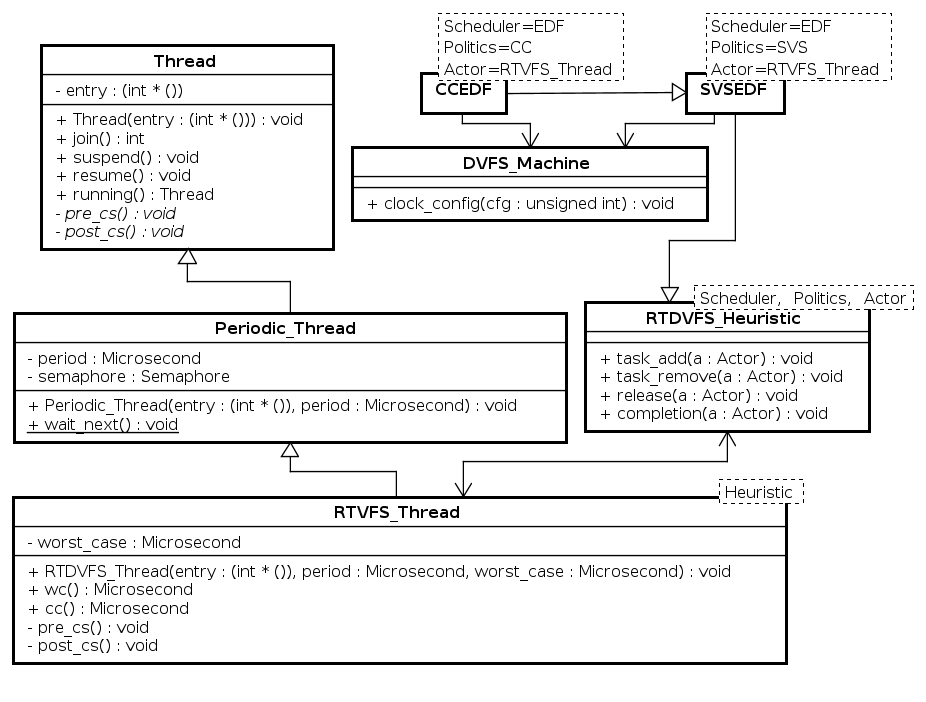
\includegraphics[scale=0.6]{imagens/ea-periodic-thread.png}
        \captionof{figure}{Diagrama de classes demonstrando as relações da \emph{EA\_Periodic\_Thread}}
        \label{fig:ea-periodic-thread}
        \end{center}
        \end{figure}
        
        Para reagir à troca de contexto, dois métodos foram criados na interface da classe \emph{Thread}: \emph{pre\_cs} e \emph{post\_cs}. Esses métodos são dedicados a extrair os pontos de execução antes e depois da troca de contexto entre \emph{threads}. Em C++, estes foram criados como funções membro virtuais, passíveis de serem sobrecarregados por classes filhas de \emph{Thread}. A interceptação destes eventos auxilia no cálculo do tempo de computação efetivamente utilizado pela tarefa.
        
        Para reagir aos outros eventos citados, a classe \emph{Periodic\_Thread} foi especializada. Uma filha chamada \emph{EA\_Periodic\_Thread} (do inglês \emph{Energy-aware Periodic Thread}) foi criada como uma abstração a fim de capturar estes eventos e repassá-los à heurística a ser utilizada. Ainda, a abstração \emph{EA\_Periodic\_Thread} recebe como parâmetros de construção o pior tempo de computação da tarefa que ela representa.
        
        \subsubsection{Captura de Modificações no Conjunto de Tarefas}
        
        A reação à alteração no conjunto de tarefas é dada a partir de duas maneiras: adição ou remoção de tarefas. Para capturar o evento de adição, em toda construção de uma nova \emph{EA\_Periodic\_Thread}, a classe \emph{Heuristic} tem o método \emph{task\_add} invocado, conforme apresentado no diagrama de sequência da figura \ref{fig:task-add}. Analogamente, na destruição de uma \emph{EA\_Periodic\_Thread}, o método \emph{task\_remove} é chamado.
        
        \begin{figure}
        \begin{center}
        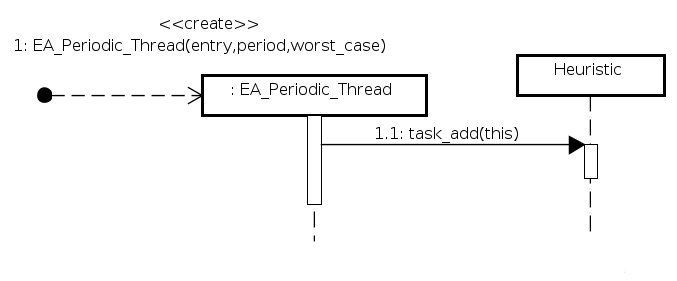
\includegraphics[scale=0.6]{imagens/task-add.png}
        \captionof{figure}{Diagrama de sequência demonstrando a criação de uma nova \emph{EA\_Periodic\-\_\-Thread}}
        \label{fig:task-add}
        \end{center}
        \end{figure}
        
        \subsubsection{Captura da Inicialização e Término de uma Tarefa}
        
        Os eventos de inicialização e término de tarefas são capturados através da reimplementação do método \emph{wait\_next} para a \emph{EA\_Periodic\_Thread}. O diagrama de sequência da figura \ref{fig:release-e-termination} mostra o momento em que estes eventos são reportados à heurística, anteriormente e posteriormente à aquisição de recurso no semáforo pertencente à \emph{thread} periódica (mecanismo explicado anteriormente na seção \ref{sec:threads-periodicas-no-epos}).
        
        \begin{figure}
        \begin{center}
        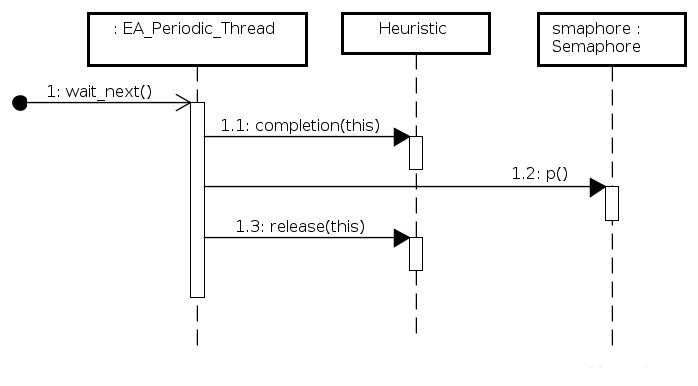
\includegraphics[scale=0.6]{imagens/release-e-termination.png}
        \captionof{figure}{Diagrama de sequência demonstrando o comportamento do método \emph{wait\_next} da classe \emph{EA\_Periodic\-\_\-Thread}}
        \label{fig:release-e-termination}
        \end{center}
        \end{figure}
        
        \subsubsection{Heurísticas}
        
        A implementação das heurísticas foram realizadas na forma de especialização de \textit{templates} em C++. A escolha da heurística pode ser programada estaticamente, sendo que cada heurística é uma especialização de três parâmetros: \emph{Scheduler} (o escalonador a ser usado, neste trabalho sempre EDF), \emph{Politics} (a política a ser utilizada: \emph{Static Voltage Scaling} ou \emph{Cycle-conserving}) e \emph{Actor} (a abstração que utiliza a heurística, neste trabalho sempre \emph{EA\_Periodic\_Thread}).
        
        \subsection{Implementação de \emph{Static Voltage Scaling} para EDF}
        
        Para implementar a heurística \emph{Static Voltage Scaling} para EDF, uma especialização \emph{SVSEDF} foi criada a partir da classe \emph{Heuristic} (figura \ref{fig:ea-periodic-thread}).
        
        A cada chamada de \emph{task\_add} ou \emph{task\_remove}, uma lista interna (\emph{periodics}) a \emph{SVSEDF} contendo objetos \emph{EA\_Periodic\_Thread} é atualizada. Quando este evento ocorre, o método \emph{select\_frequency}, escrito nos moldes do algoritmo \ref{alg:seleciona-frequencia}, é chamado. O trecho abaixo mostra o código em C++ do método citado:
        
        \begin{lstlisting}[label=select_frequency, escapeinside='', float=h, captionpos=b, caption=Método SVSEDF::select\_frequency]
        void SVSEDF::select_frequency(){
             
            EA_Periodic_Thread::List::iterator i; 
            double u = 0; // utiliza'\textit{çã}'o
            for(i = periodics.begin(); i != periodics.end(); i++){
                EA_Periodic_Thread* t = i->objetct();
                u += i->wc()/i->period();   // c'\textit{á}'lculo da utiliza'\textit{çã}'o
                                            // de pior caso
            }
            
            DVFS_Machine::Speed_Set::iterator j;
            for(j = DVFS_Machine::speed_set.begin();
                j != DVFS_Machine::speed_set.end();
                j++) {

                if(u <= j->objetct()->norm()){
                    DVFS_Machine::speed(*(j->objetct()));
                    return;
                }              
            }
            
            DVFS_Machine::speed(SVFS_Machine::max_speed());
        }
        \end{lstlisting}
        
        Observe que o método \emph{DVFS\_Machine::Speed::norm} é utilizado. Este método retorna a frequência normalizada de uma suposta configuração do tipo \emph{DVFS\_\-Machine::\-Speed}. Caso uma configuração de frequência normalizada menor ou igual a 1 não seja encontrada, a frequência máxima é utilizada.
        
        \subsection{Implementação de \emph{Cycle-conserving DVS} para EDF}
        
        Na implementação da heurística dinâmica, um método \emph{select\_frequency} também é implementado, mas neste caso, em vez do cálculo da utilização de pior caso, é feito o cálculo da utilização real quando a tarefa encontra-se terminada.

        \begin{lstlisting}[label=select_frequency, escapeinside='', float=h, captionpos=b, caption=Método CCEDF::select\_frequency]
        void CCEDF::select_frequency(){
             
            EA_Periodic_Thread::List::iterator i; 
            double u = 0; // utiliza'\textit{çã}'o
            for(i = periodics.begin(); i != periodics.end(); i++){
                EA_Periodic_Thread* t = i->objetct();
                if(!t->completed())
                    u += i->wc()/i->period();
                else
                    u += i->cc()/i->period();
            }
            
            //...
        }
        
        void CCEDF::completion(Actor* actor){
            select_frequency();
        }
        
        void CCEDF::release(Actor* actor){
            select_frequency();
        }
        \end{lstlisting}
        
        A heurística dinâmica também utiliza a adição e remoção de tarefas para atualizar a lista \emph{periodics}. Deste modo, a inicialização da execução do conjunto de tarefas sempre se dá com o processador configurado para o desempenho de pior caso de utilização. O efeito dinâmico é adquirido através da invocação de \emph{CCEDF::select\_frequency} pelos eventos de término e início de execução de das \emph{threads} periódicas.
            
            

    \chapter{Experimentos e Resultados}
    \label{chap:resultados}
    
    Este capítulo apresenta como foram conduzidos os experimentos criados para avaliar a economia de energia obtida com o ambiente RT-DVFS construído. Os resultados destes experimentos são apresentados e analisados.
    
    \section{Ambiente Experimental}
    
        O ambiente experimental foi criado com base em um conjunto pré-definido de tarefas periódicas. Como métrica para avaliação, utilizou-se a potência média de todo o sistema, composto de uma placa-mãe Gumstix Connex e sua expansão HWUART, utilizada para transmissão de dados sobre RS232.
    
    \subsection{Tarefa Canônica}
    
        Para a avaliação, uma tarefa canônica foi concebida, cujo papel é comportar-se como uma tarefa de tempo real periódica. Sua escrita em C++ dá-se como uma função não-membro que recebe como argumento dois inteiros sem sinal. O primeiro representando a ocupação da tarefa, e um segundo, representando o número de invocações que a tarefa periódica receberá, conforme mostrado no texto em C++ \ref{tarefa-canonica}.
        
        \begin{lstlisting}[label=tarefa-canonica, escapeinside='', float=t, captionpos=b, caption=Exemplo de uma tarefa canonica como uma função não-membro]
        int cononical_task(unsgiend int busy, unsigned int iterations){
            
            for(unsigned int i = iterations; i > 0; i--){
                for(volatile unsigned int b = busy; b > 0; b--);
                EA_Periodic_Thread::wait_next();
            }
            
            return 0;
        }
        \end{lstlisting}
        
        A simulação da ocupação do processador pela tarefa nada mais é do que um laço vazio, que se repete por um número constante arbitrário de vezes. Para diferentes ocupações do processador, utiliza-se diferentes constantes para a repetição do laço. Esta abordagem é a mesma utilizada no trabalho de \citeonline{Lin:2010}, onde os autores propõem um \textit{framework} destinado à avaliação de heurísticas para RT-DVFS. Vale salientar que a tarefa apresentada simula tarefas \textit{CPU-bound}, ou seja, tarefas que tem seu tempo de execução limitado principalmente pela frequência da CPU, utilizando poucas instruções que fazem acesso à memória principal.
        
    \subsection{Aplicações EPOS para Experimentação}
    
        Utilizando-se então a tarefa canônica, cinco aplicações para o sistema EPOS foram criadas, cada uma composta por três tarefas periódicas (utilizando=se a abstração \emph{EA\_Periodic\_Thread}) baseadas na tarefa canônica apresentada. As aplicações foram elaboradas para simularem 100, 80, 60, 40 e 20\% de ocupação total de CPU, sempre considerando um acréscimo de 5\% na ocupação total como sobrecarga do próprio sistema operacional e tempo de alteração de tensão e frequência para o processador. Isto significa que, uma aplicação que simula 100\% de uso, na realidade utiliza 95\% do tempo de CPU com suas tarefas. Concluindo, para uma utilização $u$, cada pior tempo de computação $C'_i$ utilizado na aplicação é na realidade $C'_i=(u-0,05u)C_i$.
        
        Para se conseguir o número de repetições do laço de cada tarefa canônica, constantes foram empiricamente aplicadas pelo programador. Utilizando-se o método \emph{cc} da abstração \emph{EA\_Periodic\_Thread}, que por sua vez utiliza o TSC do sistema, foi calculada a utilização de cada tarefa. As constantes assumidas para experimentação passaram por 10 sessões de execução por 5 segundos em configuração de frequência máxima, onde a utilização esperada pelo programador foi atingida com um desvio padrão menor que 0.01\% da média amostral. O pior tempo de computação, passado como parâmetro para a criação de cada \emph{EA\_Periodic\_Thread}, foi extraído como o maior tempo de computação obtido da amostragem citada.
        
        Cada uma das aplicações cria um conjunto de três tarefas periódicas, estas com 500, 400 e 300 milisegundos de período. A aplicação indica um número de repetições para cada tarefa, de modo que elas se repitam durante pelo menos 305 segundos. A interrupção do \emph{timer} de sistema do EPOS foi reduzido para um período de 100 milisegundos, sendo compatível com os períodos das tarefas apresentadas.
        
        Do conjunto de configurações para tensão e frequência apresentados na tabela \ref{tab:configuracoes}, o subconjunto mostrado na tabela \ref{tab:configuracoes-utilizadas} foi utilizado. Os critérios para a escolha destas configurações foram:
        
        \begin{itemize}
            \item Não há variação na frequência da memória principal, comportamento que não será avaliado neste trabalho.
            \item Para todos dispositivos que variam a frequência, o subconjunto oferece uma ordem total dos elementos (hipótese necessária para o funcionamento das heurísticas implementadas).
            \item Uniformidade (cada frequência do núcleo é um múltiplo aproximado de 0,25, ou seja, conforme a teoria apresentada na seção \ref{sec:escalonamento-em-sistemas-rt-dvfs}, há $\alpha$ 0,25, 0,50, 0,75 e 1,00).
        \end{itemize}
        
        \begin{table}
        \begin{tabularx}{\textwidth}{ |C|C|C|C| }
            \hline
            Tensão do processador ($V$)&
            Frequência do Núcleo ($MHz$)&
            Frequência do PXBus ($MHz$)&
            Frequência da SDRAM ($MHz$)\\ \hline \hline
            $1.0$ & $99,5$ & $50,0$ & $99,5$ \\ \hline
            $1.0$ & $199,1$ & $99,5$ & $99,5$ \\ \hline
            $1.1$ & $298,6$ & $99,5$ & $99,5$ \\ \hline
            $1.3$ & $398,1$ & $186,0$ & $99,5$ \\ \hline
        \end{tabularx}
        \captionof{table}{Configurações de tensão e frequência do PXA255 utilizadas nos experimentos}
        \label{tab:configuracoes-utilizadas}
        \end{table}
        
        As caches de dados e de instruções foram desligadas para a realização dos experimentos.
        
    \subsection{Configuração para Medições}
    
        Para a realização das medições, a placa Connex foi devidamente ligada à sua fonte de corrente contínua. Em seu circuito de alimentação, um resistor de 1$\Omega$ com 1\% de variação foi colocado em série com o cabo da fonte, assim como mostrado pela figura \ref{fig:setup}.
        
        \begin{figure}[h]
        \begin{center}
        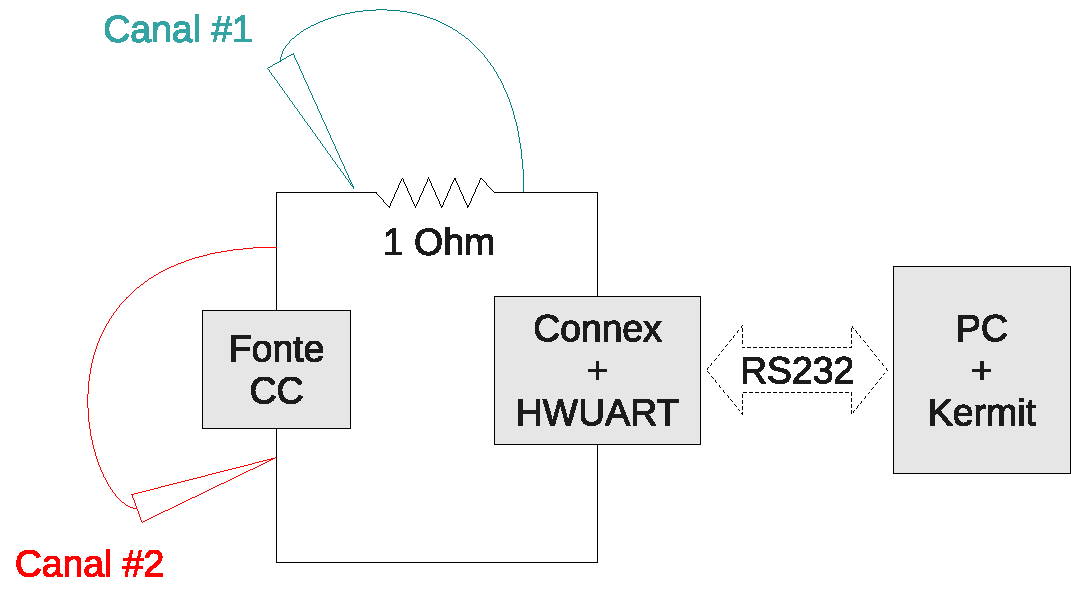
\includegraphics[scale=0.6]{imagens/setup.pdf}
        \captionof{figure}{Configuração do experimento utilizado para medições}
        \label{fig:setup}
        \end{center}
        \end{figure}
        
        Utilizando-se os canais de um osciloscópio digital, dois pontos do circuito de alimentação foram amostrados a $5Hz$: a queda de tensão no resistor apresentado e a tensão na fonte de alimentação, conforme a figura \ref{fig:setup}.
        
        A tensão medida entre as pontas do resistor, pela Lei de Ohm, pode ser convertida na corrente aproximada que passa pelo circuito. Através dessa corrente $I$ e a tensão da fonte de alimentação $U$, pode-se então ser calculada em um instante a potência $P$ dissipada pelo sistema, esta sendo $P=U\cdot I$.
        
        Para a avaliação dos resultados, a potência média $P_{med}$ foi escolhida como métrica. Sendo $U(t)$ e $I(t)$, respectivamente, a tensão e corrente do sistema no instante $t$, pode-se calcular a potência média de um instante $0$ até $T$ como sendo: $$P_{med}={1\over T}\cdot \int_{0}^{T}U(t)\cdot I(t) dt.$$
        
        A escolha da potência média como métrica deve-se ao fato de ela representar, substancialmente, o trabalho elétrico realizado por todo o dispositivo (placa-mãe e expansão). Devido à alta granularidade temporal dos eventos, a sumarização através da média não traz prejuízo à leitura do comportamento das heurísticas.
        
        Para a transmissão das aplicações à placa Connex, essa foi ligada a um PC utilizando-se o padrão RS232.
        
        \subsection{Coleta e Compilação dos Dados}
        
        As aplicações de teste foram carregadas utilizando-se a facilidade Kermit do U-Boot, como já relatado no capítulo \ref{chap:desenvolvimento}. A coleta das amostras adquiridas pelo osciloscópio foi feita através de um ``\textit{pendrive}'', no qual é possível gravar as leituras obtidas. Um programa escrito na linguagem Python foi desenvolvido com o fim de processar as amostras contidas no pendrive, calculando então a potência média utilizada para a execução das aplicações.
        
        Para cada aplicação, repetiu-se 5 vezes o processo de carregamento em memória e execução do sistema. A potência média foi calculada para estas 5 amostras, o desvio padrão manteve-se sempre entre 1\% e 2\% da potência média. Os resultados obtidos são apresentados e discutidos na seção seguinte (\ref{sec:resultados}).
    
    \section{Resultados}
        \label{sec:resultados}
        
        O gráfico apresentado na figura \ref{fig:100-100}, mostra a potência média obtida para uma utilização real igual à utilização de pior caso, ou seja, o caso onde a utilização real por cada tarefa é igual à utilização referente ao pior tempo de computação passado como parâmetro para a construção do objeto \emph{EA\_Periodic\_Thread}.
        
        \begin{figure}[h]
        \begin{center}
        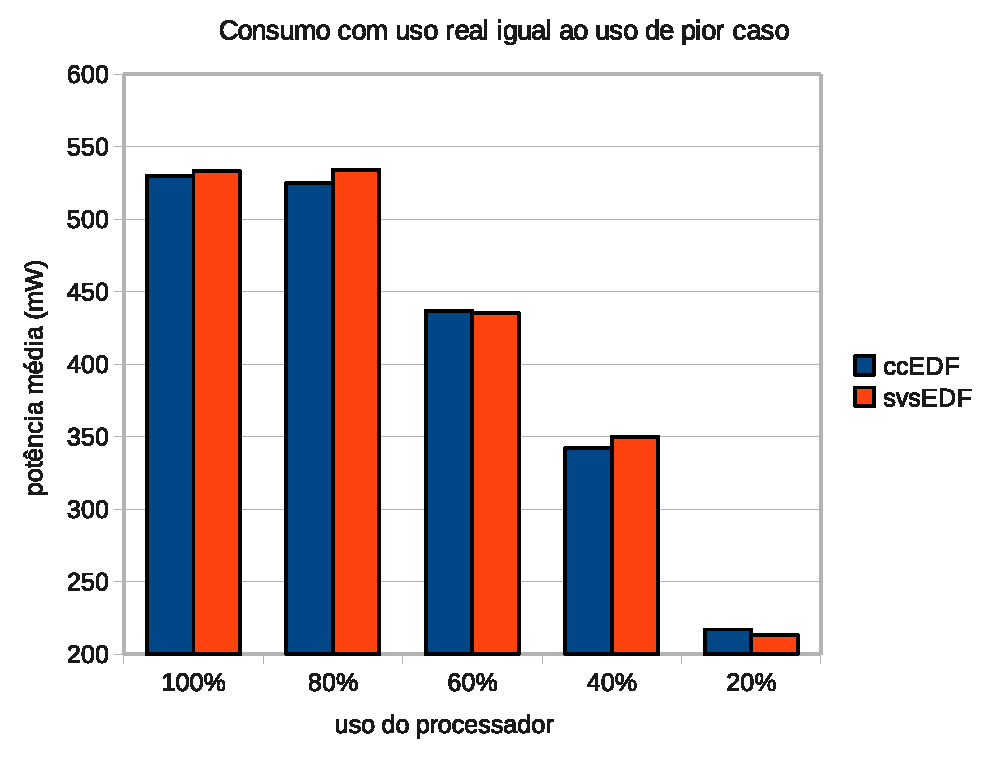
\includegraphics[scale=0.7]{imagens/grafico-100-100.pdf}
        \captionof{figure}{Gráfico da potência média com utilização real igual a de pior caso}
        \label{fig:100-100}
        \end{center}
        \end{figure}
        
        Observe que para as duas heurísticas implementadas, tanto \emph{Cycle-conserving} (ccEDF) como para \emph{Static Voltage Scaling} (svsEDF), não existe diferencial significativo no consumo entre os dois mecanismos. Isso se dá porque a heurística ccEDF tende a comportar-se como a heurística svsEDF quando a utilização real e de pior caso estão muito próximas, já que o resultado do cálculo estático e dinâmico da utilização neste caso são equivalentes. A pequena variação entre o consumo das duas heurísticas nos mesmos casos ocupação acontece devida a erros experimentais e à pequena variação presente na utilização real das tarefas.
        
        Ainda, o gráfico da figura \ref{fig:100-100} é capaz de mostrar diretamente os efeitos que as configurações de tensão e frequência causam no consumo de energia total do sistema, já que neste caso as duas heurísticas são equivalentes. A tabela \ref{tab:efeitos} apresenta a possível relação entre o uso de processador e a configuração selecionada pelo heurística estática svsEDF, segundo o que é apresentado no gráfico. Há variação na potência média para frequência normalizada 1,00 devido a erros experimentais.
        
        \begin{table}[h]
        \begin{tabularx}{\textwidth}{ |C|C|C|C|C| }
            \hline
        		Uso & Frequência de CPU & Frequência normalizada & Tensão   & Potência média \\ \hline \hline
        		$100\%$ & $398,1MHz$ & $1,00$ & $1.3V$ & $533mW$ \\ \hline   
           		$80\%$ & $398,1MHz$ & $1,00$ & $1.3V$ & $534mW$ \\ \hline
           		$60\%$ & $298,6MHz$ & $0,75$ & $1.1V$ & $435mW$ \\ \hline           		
           		$40\%$ & $199,1MHz$ & $0,50$ & $1.0V$ & $350mW$ \\ \hline
           		$20\%$ & $99,5MHz$ & $0,25$ & $1.0V$ & $213mW$ \\ \hline
        \end{tabularx}
        \captionof{table}{Relação entre uso de processador e configurações de tensão e frequência utilizadas}
        \label{tab:efeitos}
        \end{table}
        
        % É interessante observar que, mesmo não havendo queda de tensão entre os casos de 20 e 40\% de utilização, ainda há ganho energético. Teoricamente, a troca entre as configurações correspondentes a 0,25 e 0,50 de desempenho não deveria ser energeticamente eficiente. Neste experimento, acredita-se que a obtenção deste resultado é devida à redução da frequência do dispositivo PXBus, que provavelmente não oferece limites às tarefas em execução.
        
        O gráfico apresentado na figura \ref{fig:100-variando} mostra o comportamento das heurísticas com utilização de pior caso total, mas apresentando uma variação na utilização real entre 20 e 100\%. Isto significa que, mesmo as tarefas tendo como parâmetro um pior tempo de computação que causa 100\% de utilização, na realidade as tarefa canônicas correspondentes realizam apenas uma porcentagem fixa de 20 a 100\% do pior caso de computação. 

        \begin{figure}[h]
        \begin{center}
        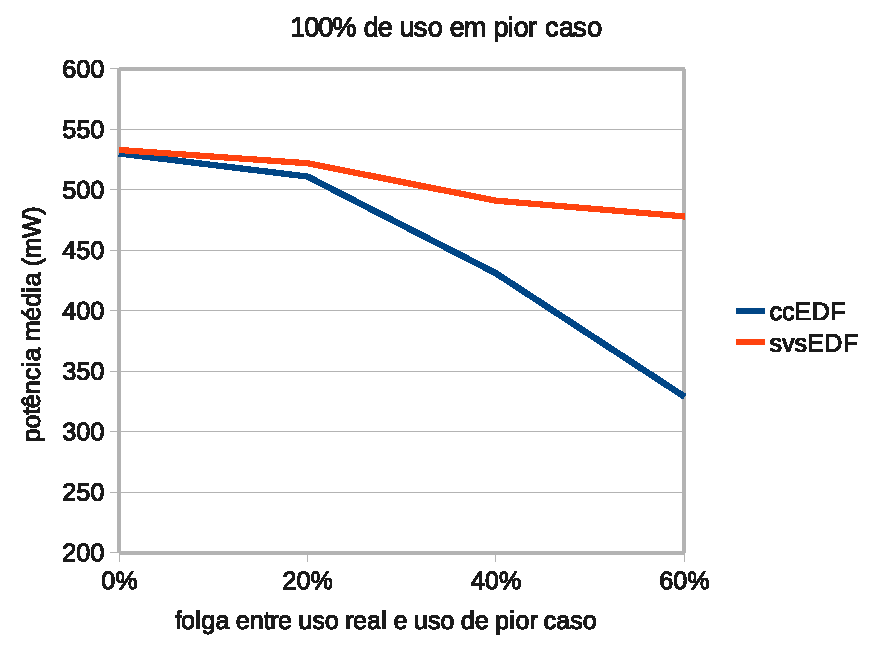
\includegraphics[scale=0.6]{imagens/100-variando.pdf}
        \captionof{figure}{Potência média em 100\% de uso de pior caso do processador com variação no uso real}
        \label{fig:100-variando}
        \end{center}
        \end{figure}
        
        A variação na utilização real apresentada demonstra a atuação da heurística dinâmica ccEDF, que leva em conta dados obtidos durante a execução do sistema. Observe que as curvas são muito próximas até a utilização real de 80\%, efeito causado pela indisponibilidade de uma configuração de tensão e frequência que represente um desempenho entre 0,75 e 1,00. O ganho só se torna observável a partir de 60\% de uso real, onde a heurística ccEDF calcula o uso dinâmico inferior ao de pior caso obtido estaticamente. A economia apresentada pela heurística estática é devido à redução no uso físico de componentes do circuito do processador.
        
        Observe que, no funcionamento da heurística dinâmica, o pior tempo de computação configurado estaticamente para cada tarefa quase sempre elevará a utilização calculada dinamicamente. O caso onde isto não acontece é quando todas tarefas foram completadas, sabendo-se o tempo de computação real utilizado por cada uma. De qualquer modo, na forma como a heurística ccEDF é escrita, este valor é ``sujado'' com o pior caso em novas requisições de tarefas. Aqui encontra-se a principal limitação da heurística \emph{Cycle-conserving}. É este tipo de problema que heurísticas de previsão (citadas na subseção \ref{sec:escalonamento-em-sistemas-rt-dvfs}) tentam resolver.
        
        \begin{figure}[h!]
        \centering
        \subfloat[]{
        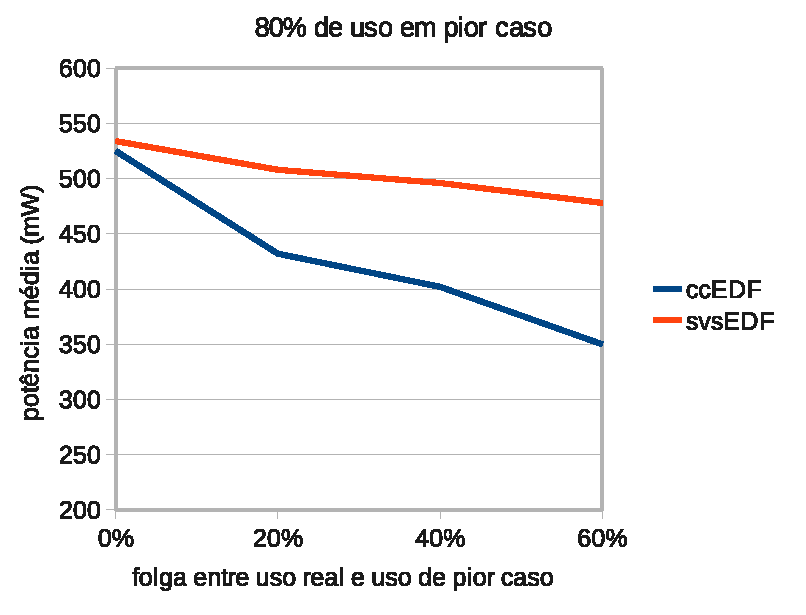
\includegraphics[scale=0.5]{imagens/grafico-80-variando.pdf}
        \label{fig:80-variando}
        }
        \subfloat[]{
        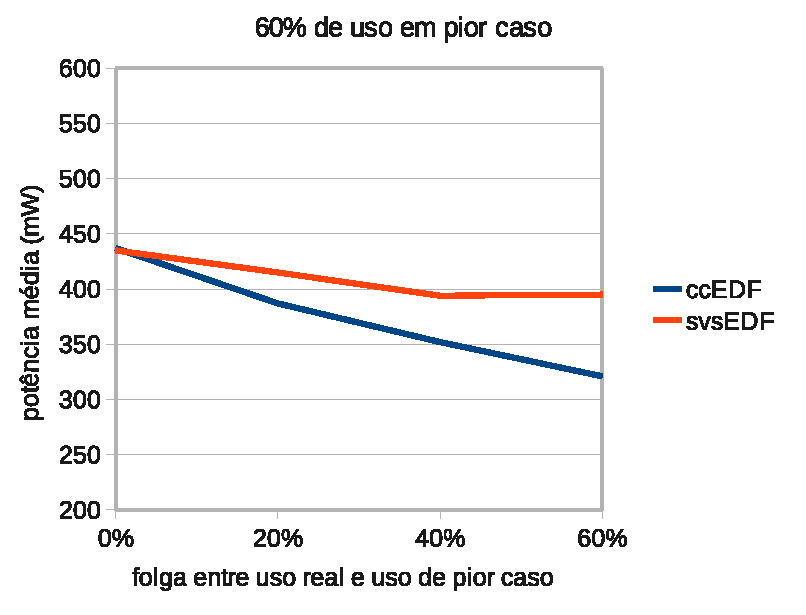
\includegraphics[scale=0.5]{imagens/grafico-60-variando.pdf}
        \label{fig:60-variando}
        }\\
        \subfloat[]{
        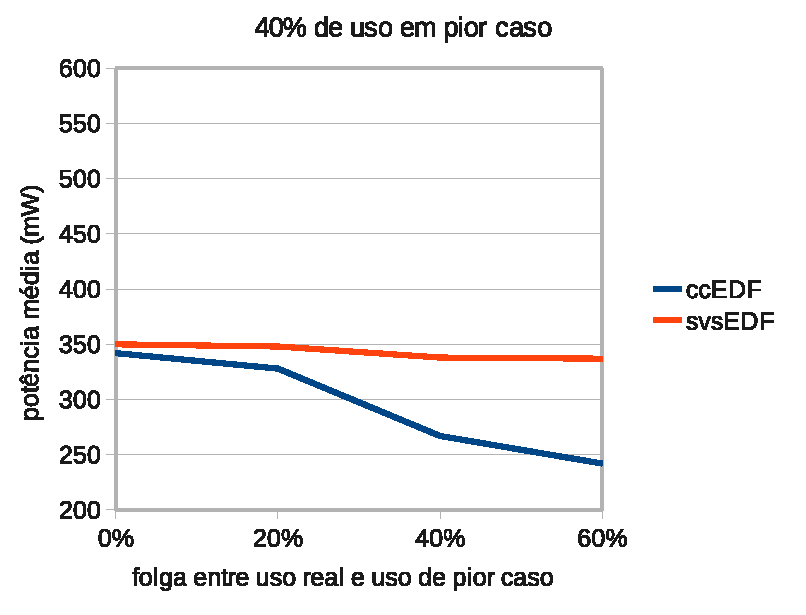
\includegraphics[scale=0.5]{imagens/grafico-40-variando.pdf}
        \label{fig:40-variando}
        }
        \subfloat[]{
        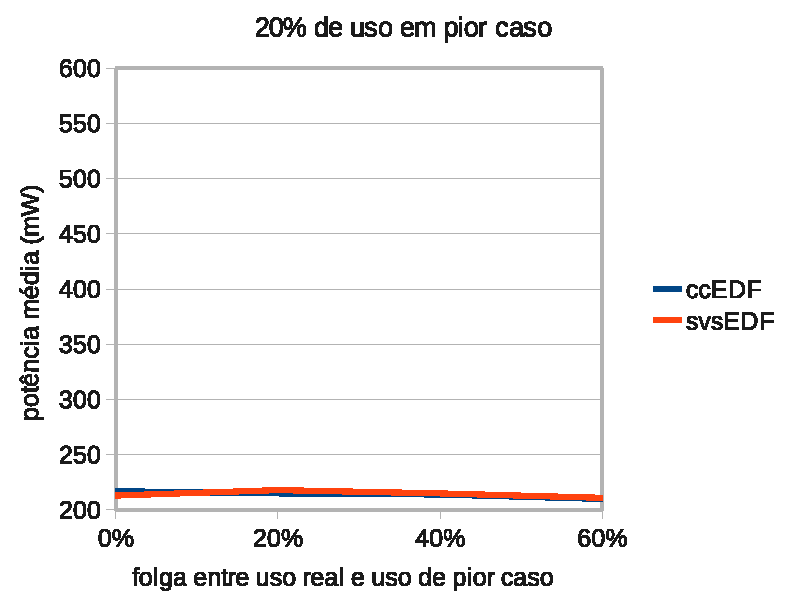
\includegraphics[scale=0.5]{imagens/grafico-20-variando.pdf}
        \label{fig:20-variando}
        }
        \caption{Potência média para uso de pior caso de 20 a 80\% com variação no uso real}
        \label{fig:80-20}
        \end{figure}
        
        O comportamento para outras utilizações de pior caso e variações no uso real, pode ser visualizado na figura \ref{fig:80-20}. É possível observar, novamente, uma queda no consumo utilizando-se a heurística svsEDF (itens \ref{fig:80-variando}, \ref{fig:60-variando}, \ref{fig:40-variando} e \ref{fig:20-variando}) isto se dá devido à redução no uso do processador. É interessante salientar que esta queda tende-se a estabilizar com redução do uso, como pode-se observar em \ref{fig:20-variando}. Isto acontece porque em d, a maior influência no consumo total do sistema passa a ser a energia estática consumida pelo PXA255, ou seja, a energia consumida não referente às consecutivas trocas de estado do circuito digital. 
        
        Ainda sobre \ref{fig:20-variando}, devido à baixa granularidade das configurações de frequência utilizadas, não há configurações de desempenho tão inferior sendo utilizadas para uso do processador inferior a 25\%, a heurística ccEDF não causa nenhuma influência.
        
        O sistema colocado em questão utilizando a heurística svsEDF pode ser entendido como um sistema de tempo real padrão com escalonamento EDF. Pode-se observar que mesmo não sendo ótima, a heurística ccEDF ainda obtém ganhos de até 25\% (na figura \ref{fig:80-variando}) neste cenário, e sem a perda de prazos. De qualquer modo, vale salientar que estes resultados sofreriam modificações caso as heurísticas fossem expostas em aplicações reais. Primeiramente, é imaginável que a folga entre uso real e de pior caso seria uma variável estocástica, como é de se esperar neste tipo de sistema. Em segundo, aplicações reais tendem a fazer um uso maior dos componentes do processador. Fatores importantes, como a influência da habilitação da memória cache do processador e aplicação de DVFS na SDRAM do PXA255 são temas para pesquisa futura.

    \chapter{Conclusão}
    \label{chap:conclusao}
    
    % não esquecer de falar dos problemas dos métodos virtuais
    % intrusão no scheduler
    % utilizar ferramentas de worst-case
    % aproveitar orientação a aplicação
    
    Os objetivos desse trabalho foram o porte do EPOS para uma plataforma de hardware com suporte a DVFS, e ainda, a implementação de técnicas para a criação de um ambiente RT-DVFS. Estes pontos foram alcançados.
    
    O EPOS agora possui um porte para o Intel PXA255, um processador com núcleo Intel XScale e suporte a DVFS para vários dispositivos internos. A plataforma é destina a aplicações de alto desempenho e baixo consumo de energia. Um fator interessante é que, agora sobre o PXA255, portar novamente o sistema para um outro processador XScale torna-se uma tarefa mais simples, já que boa parte dos mediadores referentes à arquitetura podem ser reaproveitados.
    
    As heurísticas \emph{Cycle-conserving} e \emph{Static Voltage Scaling} foram implementadas para o escalonador EDF, já presente no ambiente de tempo real do EPOS. As heurísticas implementadas foram avaliadas do ponto de vista do consumo de energia, e obtiveram o comportamento esperado para o nicho de aplicações presentes nos testes.
    
    \section{Contribuição}
    
    A maior contribuição deste trabalho encontra-se na implementação de um ambiente RT-DVFS sobre o EPOS. Grande parte das implementações de ambientes RT-DVFS utilizam o sistema operacional Linux. O EPOS é um sistema operacional nativamente desenvolvido para a produção de sistemas embarcados, além de seguir a metodologia ADESD \cite{Frohlich:2001}, um cenário diferenciado das outras implementações presentes na literatura sobre o tema.
    
    Ainda, as novas abstrações que foram criadas no sistema, permitem facilmente a criação de novas heurísticas. A classe \emph{EA\_Periodic\_Thread} é capaz de fornecer metadados referentes a execução de tarefas periódicas. Utilizando-a em conjunto com os eventos captados por \emph{Heuristic}, basta-se estender esta classe para que uma nova política para economia de energia seja adicionada ao sistema. Vale salientar que, como proposto por \citeonline{Pillai:2001}, as heurísticas continuam fracamente acopladas ao escalonador de tempo real do sistema operacional embarcado.
    
    \section{Trabalhos Futuros}
    
    Mesmo que com seus objetivos cumpridos, este trabalho ainda necessita de amadurecimento em um aspecto principal: \emph{design} de software.
    
    A abstração \emph{Thread} do EPOS não permite captar os eventos de troca de contexto. O conceito utilizado neste trabalho para trabalhar com estes eventos foi a adição de polimorfismo dinâmico na classe \emph{Thread}, o que leva a indireções no controle de fluxo da troca de contexto. Esta foi a alternativa utilizada pois o EPOS ainda utiliza \emph{threads} não periódicas para representar a \emph{thread} principal do sistema e a \emph{thread} que ocupa o processador em inatividade. Procurar uma alternativa ``mais estática'' provavelmente recairia em um reprojeto maior do sistema, o que está fora do escopo deste trabalho. Observe que a captura deste tipo de evento é interessante para adicionar flexibilidade para a criação de novas abstrações de processos no EPOS.
    
    Além disso, como trabalhos futuros, ainda aponta-se:
    \begin{itemize}
        \item Criar experimentos com aplicações mais complexas ou reais. O estudos em RT-DVFS revelam que a realidade para tarefas que tem um uso maior da memória é outra, como apresentando por \citeonline{Snowdown:2005}. 
        \item Realizar experimentos comparativos com as implementações existentes sobre Linux.
        \item Já que o EPOS é orientado a aplicação, poderia-se realizar uma análise estática ou dinâmica a fimde presumir mecanismos ou parâmetros de heurísticas para RT-DVFS.
    \end{itemize}
    
    



    \bibliography{../bibliografia}

    %\apendice
    %\include{apendices}
    
\end{document}
